\documentclass[journal]{IEEEtran}

\usepackage[numbers,sort,compress]{natbib}
\usepackage{bm}
\usepackage{amsmath}
\usepackage{amssymb}
\setcounter{tocdepth}{3}
\usepackage[pdftex]{graphicx}

\usepackage{epstopdf}
\usepackage{url}
\usepackage{hyperref}
\usepackage[boxed]{algorithm2e}
\usepackage{xcolor}

\usepackage{placeins}

\usepackage[T1]{fontenc}
%\usepackage{caption}
%\usepackage{subcaption}
\usepackage[caption=false,justification=centerlast,singlelinecheck=false]{subfig}	%subcaption/subfigure are deprecated
                                    % 'caption' not recommended by package

\newcommand{\comment}[1]{\textcolor{red}{#1}}
\newcommand{\note}[1]{\textcolor{blue}{#1}}

\newcommand{\di}[2]{\frac{\partial#1}{\partial#2}}
\newcommand{\trans}[1]{#1^{\scriptscriptstyle T}}
\newcommand{\trace}{\mathrm{tr}}
\newcommand{\diag}{\mathrm{diag}}
\newcommand{\kron}{\mathrm{kron}}
\DeclareMathOperator*{\argmin}{arg\,min}

\graphicspath{{./}{./images/}}	% paths for images
\DeclareGraphicsExtensions{.pdf,.png,.jpg}  % extensions, in order of preference
\begin{document}

\title{Joint Biomechanical Surface Registration: Application to MR-TRUS Fusion for Prostate Interventions}

\author{Siavash~Khallaghi, C.~Antonio~Sanchez, Abtin~Rasoulian, Saman~Nouranian, Hamidreza~Abdi, Silvia~D.~Chang, Aaron~Fenster, Aaron~Ward, Sidney~Fels and Purang~Abolmaesumi% <-this % stops a space
\thanks{Siavash Khallaghi, C.~Antonio~Sanchez, Abtin~Rasoulian, Saman~Nouranian, Sidney~Fels and Purang~Abolmaesumi are with the Department of Electrical and Computer Engineering, University of British Columbia, Vancouver, BC, Canada.}%
\thanks{Hamidreza~Abdi and Silvia~D.~Chang are with the Vancouver General Hospital, Vancouver, BC, Canada.}%
\thanks{Aaron~Fenster and Aaron~Ward are with the University of Western Ontario, London, ON, Canada.}%
\thanks{Manuscript received Month XX, Year; revised Month XX, Year.}}

\markboth{IEEE TRANSACTIONS ON MEDICAL IMAGING, VOL. XX, NO. X, Month~Year}%
{S. Khallaghi \MakeLowercase{\textit{et al.}}: Joint Biomechanical Partial Surface Registration...}

% make the title area
\maketitle

\begin{abstract}
We present a novel non-rigid surface registration method for two partial surfaces. Our approach incorporates prior geometrical and physical knowledge in a probabilistic registration framework. We validate results in the context of prostate interventions on pre-operative magnetic resonance imaging (MRI) and 3D transrectal ultrasound (TRUS) data acquired from prostate biopsy patients. We show that both geometrical and physical priors are required in order to decrease the target registration error (TRE). We demonstrate an improvement of $1.95$~mm and $1.78$~mm following the proposed registration approach on full and partial surfaces, respectively. We investigate the robustness of our approach by removing entire portions of the prostate surface in different areas. Our results show that the proposed surface registration is a promising technique.
\end{abstract}

\begin{IEEEkeywords}
Statistical shape model, Gaussian mixture model, finite element modeling, surface registration, prostate, biopsy.
\end{IEEEkeywords}

\IEEEpeerreviewmaketitle
%%%%%%%%%%%%%%%%%%%%%%%%%%%%%%%%%%%%%%
\section{Introduction}
%%%%%%%%%%%%%%%%%%%%%%%%%%%%%%%%%%%%%%
\IEEEPARstart{I}{mage} guided interventions (IGI), often require the registration of pre-operative (pre-op) images to intra-operative data. Pre-op imaging, often done through computed tomography (CT) and magnetic resonance imaging (MRI), provides information about the patient anatomy, location and extent of the disease. A popular choice of intra-operative (intra-op) imaging is ultrasound (US), which is a low-cost, real-time and radiation-free modality widely used for abdominal and urological interventions. Since the pre-op and intra-op images are acquired in two different physical spaces, some form of registration is required to establish the relationship between the two in patient coordinates.

Registration of pre-op and intra-op images is inherently challenging. In many applications, the anatomy of interest undergoes motion and changes shape due to different body positions between acquisitions. As a result, the registration needs to solve for a six degree-of-freedom transform for rigid and a much larger parameter space for non-rigid applications. The large number of parameters often results in an ill-posed problem according to Hadamard's definition~\cite{Hadamard23}.

Non-rigid multi-modality intensity-based registration is an active field of research~\cite{Pluim03a,Sotiras13a}. Recently, a new feature-set, \textit{modality independent neighborhood descriptor} (MIND), was proposed based on denoising literature~\cite{Heinrich12a}. The extension of this framework has been successfully used for multi-modal prostate registration using dual-prime optimization~\cite{Sun13a}. However, similar to all intensity-based approaches, MIND still requires anatomical features to appear in both images~\cite{Heinrich12a}. This may be challenging when imaging physics are substantially different between two modalities, which results in parts of the anatomy to be invisible in one image. For example, the TRUS boundary of the prostate is not easily visible in the base to the point that it is often difficult to tell where the prostate ends and seminal vesicles begin.

If both the pre-operative and intra-operative images are segmented during the clinical workflow, we can bypass difficulties associated with multi-modal intensity-based registration through a surface-based method. However, especially for prostate interventions, even experts are prone to over and under segmentation of the anatomy~\cite{Smith07a}. Parts of the boundary may not even be visible in one or both modalities. Thus, in the general case, the solution requires the registration of two partial surfaces. The main topic and contribution of this paper is to propose an elegant and efficient way to register two surfaces together where both surfaces are only partially segmented.
%%%%%%%%%%%%%%%%%%%%%%%%%%%%%%%%%%%%%%
\subsection{Literature Review}
%%%%%%%%%%%%%%%%%%%%%%%%%%%%%%%%%%%%%%
Surface-based registration of a source, $Y$, and a target surface, $X$, is often presented as the minimization of an objective functional of the form
%%%%%%%%%%%%%%%%%%%%%%%%%%%%%%%%%
\begin{equation} \label{eq:SurfReg}
\mathcal{E}(X,T(Y,\Theta))+\mathcal{R}(\Theta).
\end{equation}
%%%%%%%%%%%%%%%%%%%%%%%%%%%%%%%%%%%%%%
The first term, $\mathcal{E}(.)$, is a distance metric between source and target surfaces given a transformation, $T(.)$, parameterized by $\Theta$. The second term, $\mathcal{R}(.)$, is a regularization term that seeks to constrain specific properties in the solution that the user requires. For non-rigid registration, regularization dictates the nature of the transformation as well.

The distance metric in surface-based techniques is typically formulated as a summation of distances between corresponding points. Thus, the metric and the correspondence scheme are intimately related. The closest point criterion, used in the iterative closest point (ICP) algorithm~\cite{Besl92a,Zhang94a} is one of the most popular approaches. However, ICP requires accurate initialization to converge and is very sensitive to noise, outliers and missing surface points. 

In order to address these issues, soft-correspondences have been proposed, where the registration is cast to the estimation of the parameters of a Gaussian Mixture Model (GMM)~\cite{Chui03a,Wang08a,Jian11a,Myronenko10a,Horaud11a}. However, even though these methods are robust to missing observations in the target surface, they assume a complete source surface without any missing points. When both surfaces are only partially segmented, more informed priors are required to tackle the underdetermined nature of the registration problem. 

A standard approach in gathering prior knowledge is through statistical modeling of a population of training shapes, known as a statistical shape model (SSM)~\cite{Heimann09a}. Compared to intensity-based SSMs~\cite{Avants04a,Balci07a,Bhatia04a,Cootes08a,Joshi04a,Rueckert03a,Twining05a,Wang10a}, the literature is very sparse in the generation of their surface-based counterparts~\cite{Chui04a,Davies02a,Durrleman09a,Rasoulian12b}. In the landmark paper by Cootes~\textit{et~al.}~\cite{Cootes95a}, a manual correspondence scheme is used, which is tedious, time-consuming and subject to user variability. To address these issues, pair-wise construction techniques have been proposed, where one shape is arbitrarily chosen as the mean and registered to all other shapes in the training set. Unfortunately, this approach is inherently biased towards the selected mean-shape, which may reduce the generality of the resulting SSM. In order to remove this bias, group-wise registration techniques have been developed~\cite{Balci07a,Rasoulian12b}, where both the mean-shape and its pair-wise transformation are considered unknown. 

If a general, specific and compact surface-based SSM of the anatomy is available, it is possible to perform partial-surface to partial-surface registration through this statistical representation. This reformulates the original problem as a full-surface to two partial-surfaces registration, which is, hopefully, no longer underdetermined. In this approach, the SSM is considered the source, and both partial surfaces are considered target surfaces. However, in probably all deformable organs, the two partial surfaces are in a different biomechanical state compared to both each other and the SSM. As a result, in addition to SSM parameters that control the model shape, the registration needs to solve for an additional non-rigid transformation between the SSM and the two partial surfaces. Furthermore, since the interior of the anatomy is typically the region of interest during an IGI, this additional non-rigid registration needs to be volumetric. The rest of this section describes popular non-rigid transformation models in the literature: 1) Geometric-inspired; 2) Interpolation-inspired; and 3) Knowledge-based models.

Geometric-inspired models provide a minimal set of properties that are intuitively common when similar objects are mapped together. Such properties include, but are not limited to, inverse consistency~\cite{Combes10a}, topology preservation~\cite{Huang07a,Yeo10a,Moradi12a} and isometry~\cite{Zheng10a}. To the best of our knowledge, the only geometric-inspired approach for prostate interventions is the method by Moradi~\textit{et~al}~\cite{Moradi12a}. While they achieve a registration accuracy of $3.2$~mm, their method is still sensitive to contiguous regions around the apex where the prostate contour has poor visibility~\cite{Moradi12a}. 

Interpolation-inspired models assume that there is an error in the estimation of displacements. Thus, the transformation smoothly approximates the known displacements rather than taking the exact same values. Examples of important families of interpolation strategies include radial basis functions~\cite{Chui03a}, free-form deformations~\cite{Wang08a} and Gaussian basis functions~\cite{Myronenko10a}. These methods have been used for statistical shape analysis~\cite{Zhang13a,Rasoulian12b,Achuthan13a} and prostate interventions~\cite{Makni10a,Makni12a}. However, in these methods only surface displacements are regularized and volumetric deformations can only be is recovered via post-registration interpolation. This may result in unnatural changes in shape, since the interior deformation field is not directly regularized during the course of the registration.

Knowledge-based transformation models are typically used in scenarios that involve a well-defined task for a specific organ. Introducing knowledge regarding the deformation may be achieved in two ways, statistical analysis and biomechanical modeling. Similar to SSMs, statistical deformation models (SDMs) capture statistical
information about deformation fields across an initial population. For a new subject, the registration strives to find a linear combination of SDM basis transforms that minimizes an objective functional~\cite{Hu12a,Ashraf02a}. The drawback of SDMs is that they require an additional training step, and their capture range is limited to previously-observed deformations~\cite{Hu12a}.

The main motivation behind biomechanical modeling is the premise that physically consistent models allow a more accurate description of complex deformation fields.
Usually, finite element methods (FEMs) are employed to model biomechanical properties of deformable organs. During registration, the biomechanical model is used to update the entire deformation field using a combination of pseudo-forces and boundary conditions~\cite{Cash05a,Ferrant01a,Moradi12a,Noe10a,Rucker14a}. To model forces, typically a variation of ICP is used~\cite{Ferrant01a,Moradi12a,Rucker14a}, which is susceptible to the drawbacks of these local-search techniques. Rather than using ICP, we combine the geometrical and biomechanical priors into a single framework using a global probabilistic approach.
%%%%%%%%%%%%%%%%%%%%%%%%%%%%%%%%%%%%%%
\subsection{Contributions}
%%%%%%%%%%%%%%%%%%%%%%%%%%%%%%%%%%%%%%
In this work, we aim to improve the accuracy of IGIs by developing a new non-rigid surface-based registration framework (joint SSM-FEM) that considers the geometrical statistics and biomechanical nature of the deformation between pre-operative and intra-operative acquisitions. To compensate for potential difficulties in segmentation, we propose to segment the anatomy in each image only where the boundary can be reliably and precisely traced. This results in two partial segmentations of the anatomy, which are then concurrently fused through a SSM. In order to model residual biomechanical deformations, a FE model is used.

The basic idea is similar to Rasoulian~\textit{et~al.}~\cite{Rasoulian13a}, where a SSM is used to capture the bulk of shape appearances and a smooth non-rigid transformation is used to compensate for residual errors. However, in our case, the SSM is jointly registered to two partial observations of the anatomy and the nature of the subsequent non-rigid transformation is biomechanical. Our approach differs from linked statistical shape models (LSSMs)~\cite{Chowdhury12a} since we also solve for the volumetric deformation field interior to the surfaces. We validate our registration algorithm in the context of MR-TRUS fusion on ten patients who underwent a prostate biopsy. We validate our registration method with and without the geometrical and biomechanical priors. This helps demonstrate the need for SSM and FEMs when dealing with missing data in elastic surfaces.
%%%%%%%%%%%%%%%%%%%%%%%%%%%%%%%%%%%%%%
\begin{figure*}[t]
\center
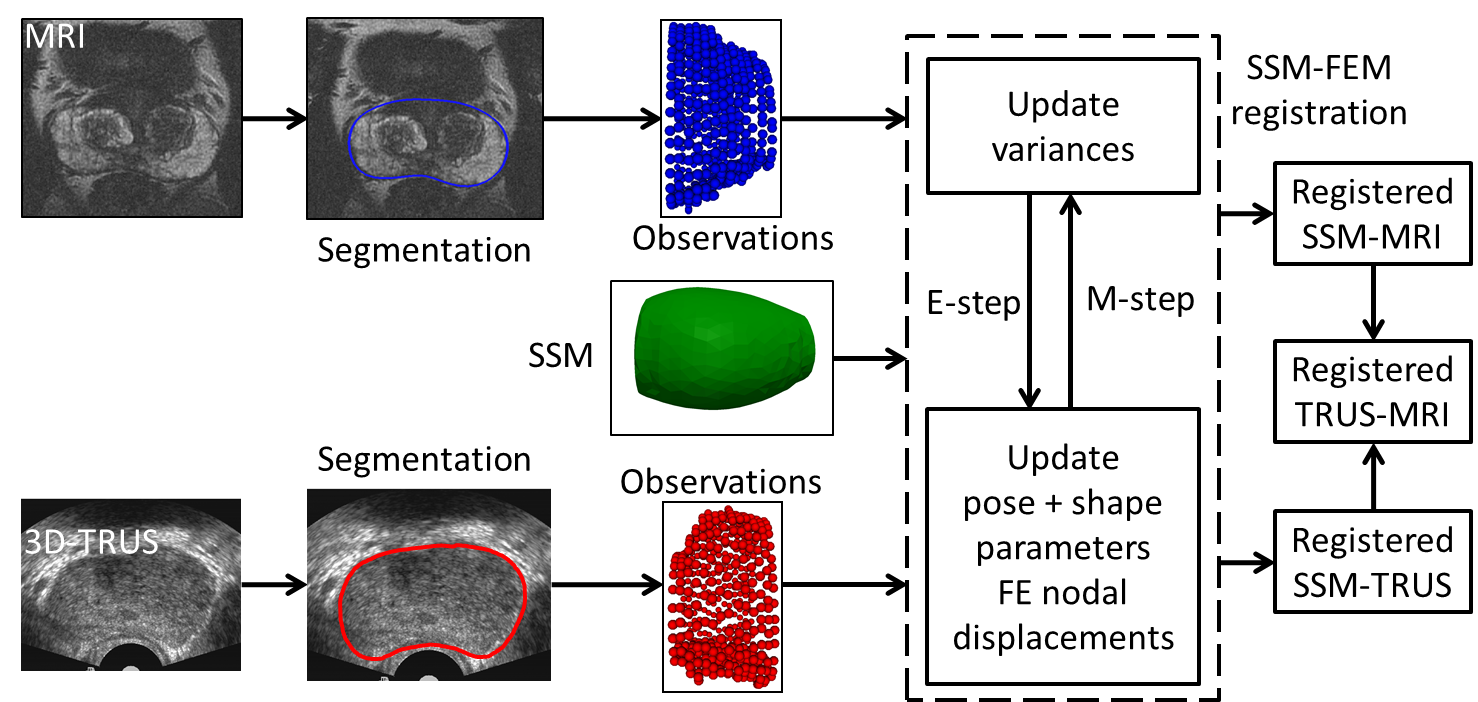
\includegraphics[width = 0.65\textwidth]{images/workflow.png}
\caption{Overview of the registration framework. The pre-operative (MR) image is taken before the procedure and is segmented to create a surface representation of the anatomy, in this case the prostate. At the beginning of the procedure, an intra-operative (3D-TRUS) image is acquired and parts of the anatomy (midgland) are segmented. The SSM-FEM registration maps both surfaces and their interior to the common SSM representation. Subsequently, the MRI is registered to the TRUS space by concatenating MRI-SSM and TRUS-SSM transforms.}
\label{fig:workflow}
\end{figure*}
%%%%%%%%%%%%%%%%%%%%%%%%%%%%%%%%%%%%%%
\section{Method}
%%%%%%%%%%%%%%%%%%%%%%%%%%%%%%%%%%%%%%
An outline of our proposed joint SSM-FEM registration approach is shown in Figure~\ref{fig:workflow}. The partial-surface-to-partial-surface registration is cast to two SSM-to-partial-surface problems, which are solved concurrently using an expectation-maximization (EM) algorithm. In our formulation, the SSM is used to construct two probability density functions (one for each modality) for defining the boundary of the structure, and the other two segmented surfaces are considered as two sets of observations. The two probability density functions relate the SSM to surface points in each modality. We wish to find two sets of transformations that maximizes the likelihood that the observations came from the transformed probability distributions.

To construct the SSM, we used our previously developed group-wise GMM approach, which has been shown to provide a general, specific and compact representation of genus-zero surfaces~\cite{Rasoulian12b}. Details of the training are provided in Section~\ref{sec:ssm}. We refer to a linear combination of weights, hereafter referred to as \textbf{shape parameters}, and modes of variation as an \textbf{instance} of the SSM. The parameters that control the rigid transformation of an instance are referred to as \textbf{pose parameters}. During the course of registration, instances of the SSM are used to create a FE model of the prostate. This FE model is used to calculate internal deformations given surface-driven forces. Note that to form an FE model from a surface, we often need to add interior nodes. This can be done with most FE-meshing tools, such as TetGen \cite{Si06a}.

To define the probability distribution for each modality, we use a GMM, which has been widely used to establish soft correspondences~\cite{Myronenko10a,Rasoulian12a,Jian11a}. A GMM is a parametric probability density function represented as a weighted sum of Gaussian densities. Vertices of the SSM mean are assumed to be the centroids of Gaussian components, each represented by a mean and a variance. For simplicity, we take the variance to be isotropic in all directions for all components.

The key idea in our registration is that the points on the surface of the prostate in US and MR are deformed observations of a common instance of the SSM. Hence, the solution to the shape parameters depend on both sets of observations. For simplicity, we consider the pose and biomechanical parameters between the SSM and each group of observations to be independent of each other. A full list of notations for the proposed joint SSM-FEM method is presented in Table~\ref{tbl:notation}.
%%%%%%%%%%%%%%%%%%%%%%%%%%%%%%%%%%%%%%
\begin{table}[!bht]
  \centering
  \caption{Mathematical Notations \label{tbl:notation}}
  \begin{tabular}{lp{0.55\columnwidth}}
  \hline
    $\mathrm{md}\in\{\mathrm{US},\mathrm{MR}\}$ & Modality\\
    $D$ & Dimension of the surfaces\\
    $N_\mathrm{md},M,L,J$ & Number of observations in modality, SSM nodes, modes of variation and FEM nodes\\
    $X_\mathrm{md}$ & ${N_\mathrm{md}\times D}$ Observations\\
    $Z_{M\times D}$ & SSM mean\\
    $\Psi_{DM\times L}$ & Modes of variation in rasterized format\\
    $b_{L\times 1}$ & Shape parameters\\
    $R_\mathrm{md},t_\mathrm{md},s_\mathrm{md}$ & $D\times D$ Rotation, $D\times 1$ translation and scale\\
    $Y_{M\times D}$ & An instance of the SSM\\
    $U_\mathrm{md}$ & ${J\times D}$ FEM nodal displacements\\
    $x^\mathrm{md}_n$ & n-th point of observations\\
    $z_m$ & m-th SSM mean node\\
    $y_m$ & m-th instance node\\
    $\vec{v}_{DN \times 1}$ & Rasterized representation of a $V_{N\times D}$ matrix\\
    $\Phi_{M\times J}$ & FEM interpolation matrix\\
    $K$ & Stiffness matrix\\
    $E$ & Young's modulus\\
    $\nu$ & Poisson's ratio\\
    $P_{\mathrm{md}}$ & $M\times N_\mathrm{md}$ GMM posterior probabilities\\ 
    $\sigma_{\mathrm{md}}^2$ & Variance of Gaussian components\\
    $0{\leq}w_{\mathrm{md}}{\leq}1$ & Estimate of outliers/missing data\\
    $\diag{(\vec{v})}$ & Diagonal matrix of a vector $\vec{v}$\\
    $I$ & Identity matrix\\
    $\tilde{P} = \kron{(P,I_{D\times{D}})}$ &Kronecker product of $P$ and $I$\\
    $1$ & Column vector of all ones\\
    \hline\\
  \end{tabular}
\end{table}
%%%%%%%%%%%%%%%%%%%%%%%%%%%%%%%%%%%%%%
\subsection{Joint SSM-FEM Registration}
%%%%%%%%%%%%%%%%%%%%%%%%%%%%%%%%%%%%%%
The joint SSM-FEM registration, hereafter referred to as SSM-FEM registration, is constrained by Tikhonov regularization over shape parameters and the volumetric strain energy of an FE model. The solution to the rigid transforms, shape parameters and nodal displacements are derived using implicit surface-to-surface forces, from the SSM to each set of observations. These forces arise naturally by minimizing the following objective functional:
%%%%%%%%%%%%%%%%%%%%%%%%%%%%%%%%%%%%%%
\begin{equation} \label{eq:objTotal1}
\mathcal{E} = \sum_{\mathrm{md}\in\{\mathrm{MR},\mathrm{US}\}}\mathcal{E}_\mathrm{md}(\sigma^2_\mathrm{md},\Theta_\mathrm{md}),
\end{equation}
%%%%%%%%%%%%%%%%%%%%%%%%%%%%%%%%%%%%%%
where $\Theta_\mathrm{md}=(R_\mathrm{md},t_\mathrm{md},s_\mathrm{md},U_\mathrm{md},b)$ is the concatenation of the rigid transform, shape parameters and nodal displacements. Shape parameters do not have a modality subscript, since we take them to be common between the two observations. $\mathcal{E}_\mathrm{md}(.)$ is the negative log-likelihood function defined as:
%%%%%%%%%%%%%%%%%%%%%%%%%%%%%%%%%%%%%%
\begin{multline} \label{eq:objMod1}
\mathcal{E}_\mathrm{md}(\sigma^2_\mathrm{md},\Theta_\mathrm{md}) = \\ -\sum_{n=1}^{N_\mathrm{md}}\log\sum_{m=1}^MP_\mathrm{md}(z_m)P_\mathrm{md}(x^\mathrm{md}_n|T(z_m,\Theta_\mathrm{md})),
\end{multline}
%%%%%%%%%%%%%%%%%%%%%%%%%%%%%%%%%%%%%%
where $P_\mathrm{md}(\cdot)$ denotes the GMM probability density function~\cite{Myronenko10a} and $T(z_m,\Theta_\mathrm{md})$ represents the concatenated transformation at the m-th SSM node. This transform is defined as:
%%%%%%%%%%%%%%%%%%%%%%%%%%%%%%%%%%%%%%
\begin{equation} \label{eq:concTransform1}
T(z_m,\Theta_\mathrm{md}) = s_\mathrm{md}R_\mathrm{md}(y_m+v^\mathrm{md}_m) + t_\mathrm{md},
\end{equation}
%%%%%%%%%%%%%%%%%%%%%%%%%%%%%%%%%%%%%%
where $y_m=z_m+\Psi_mb$ represents the m-th instance node given shape parameters and corresponding elements in $\Psi$. $v^\mathrm{md}_m$ is the residual biomechanical deformation between the instance and observations in each modality. Since the SSM is a surface model, we use an interpolation matrix $v^\mathrm{md}_m=\Phi_mU_\mathrm{md}$ to relate surface displacements to nodal displacements. In our implementation, all points on the surface correspond to FE nodes, and internal nodes are appended to the end of the node list. As a result, the interpolation matrix has the form, $\Phi=\begin{bmatrix} I_{M\times M} & 0\\ 0 & 0 \end{bmatrix}$. Hence, we can expand Equation~\ref{eq:concTransform1} as
%%%%%%%%%%%%%%%%%%%%%%%%%%%%%%%%%%%%%%
\begin{equation} \label{eq:concTransform2}
T(z_m,\Theta_\mathrm{md}) = s_\mathrm{md}R_\mathrm{md}(z_m+\Psi_mb+\Phi_mU_\mathrm{md})+t_\mathrm{md}.
\end{equation}
%%%%%%%%%%%%%%%%%%%%%%%%%%%%%%%%%%%%%%
Subsequently, the unknowns, i.e. $\sigma^2_\mathrm{md}$ and $\Theta_\mathrm{md}$, are solved using an EM algorithm. Initially, the variance is estimated as Myronenko~\textit{et~al.}~\cite{Myronenko10a}
%%%%%%%%%%%%%%%%%%%%%%%%%%%%%%%%%%%%%%
\begin{equation} \label{eq:initVariance}
\sigma^2_\mathrm{md} = \frac{1}{DMN_\mathrm{md}}\sum_{n=1}^{N_\mathrm{md}}\sum_{m=1}^{M}\left\|x^{\mathrm{md}}_n-z_m\right\|^2.
\end{equation}
%%%%%%%%%%%%%%%%%%%%%%%%%%%%%%%%%%%%%%
In the expectation step, we compute how likely an observation corresponds to a GMM centroid by calculating the posterior probability
%%%%%%%%%%%%%%%%%%%%%%%%%%%%%%%%%
\begin{equation} \label{eq:prob}
P_\mathrm{md}(z_m|x^\mathrm{md}_n) = \frac{\exp{\left(-\frac{1}{2}\frac{\left\|x^\mathrm{md}_n -T(z_m,\Theta_\mathrm{md})\right\|^2}{\sigma^2_\mathrm{md}}\right)}}{\sum_{j=1}^M\exp{\left(-\frac{1}{2}\frac{\left\|x_n -T(z_j,\Theta_\mathrm{md})\right\|^2}{\sigma^2_\mathrm{md}}\right)} + c},
\end{equation}
%%%%%%%%%%%%%%%%%%%%%%%%%%%%%%%%%
where $c=(2\pi\sigma^2_\mathrm{md})^{D/2}\frac{w_\mathrm{md}}{1-w_\mathrm{md}}\frac{M}{N_\mathrm{md}}$ is the contribution of an additional uniform distribution to account for noise, outliers and missing data. $0{\leq}w_\mathrm{md}{\leq}1$ controls the weight of equal membership probabilities, set to zero if observations do not exhibit any noise, outliers or missing data. A value of one denotes that no correspondence between observations and GMM centroids can be made. Ignoring constants independent of $\sigma^2_\mathrm{md}$ and $\Theta_\mathrm{md}$, we can rewrite the maximization step of Equation~\eqref{eq:objMod1} with an added Tikhonov and FE regularizer:
%%%%%%%%%%%%%%%%%%%%%%%%%%%%%%%%%
\begin{multline} \label{eq:objMod2}
Q(\sigma^2_\mathrm{md},\Theta_\mathrm{md}) = \frac{N^\mathrm{md}_PD}{2}\log(\sigma^2_\mathrm{md})\\
+ \frac{\mu}{4}\trans{b}\Lambda{b} + \frac{\beta}{2}\trans{\vec{u}_\mathrm{md}}K\vec{u}_\mathrm{md}\\
+ \frac{1}{2\sigma^2_\mathrm{md}}\sum_{m,n=1}^{M,N_\mathrm{md}}P_\mathrm{md}(z_m|x^\mathrm{md}_n)\left\|x^\mathrm{md}_n- T(z_m,\Theta_\mathrm{md})\right\|^2,
\end{multline}
%%%%%%%%%%%%%%%%%%%%%%%%%%%%%%%%%
where $N^\mathrm{md}_P=\sum_{m,n=1}^{M,N_\mathrm{md}}P_\mathrm{md}(z_m|x^\mathrm{md}_n)$. The $\mu$ parameter controls the Tikhonov regularizer on shape parameters and $\Lambda$ is the diagonal matrix of inverted SSM eigenvalues. The $\beta$ parameter controls the trade-off between the tightness of the fit and biomechanical regularization. This regularizer represents the total strain energy of the FE model. 

The FE regularizer is derived from a linear stress-strain relationship. Given a set of nodal displacements, $\vec{u}$, the forces acting on the nodes due to internal strain are given by $\vec{f} = K\vec{u}$, where $K$ is known as the \emph{stiffness matrix} \cite{Bonet00a}.  This large sparse matrix can be systematically constructed based on the FE mesh and the linear material model.  The internal energy of the system is then given by $\frac{1}{2}\trans{\vec{u}}\vec{f}=\frac{1}{2}\trans{\vec{u}}K\vec{u}$, which is exactly the cost for the FEM-based regularization term in the equation above. In the current implementation, we remesh the prostate to create an FE model every time a new instance is created. Substituting Equation~\ref{eq:objMod2} into Equation~\ref{eq:objTotal1} yields:
%%%%%%%%%%%%%%%%%%%%%%%%%%%%%%%%%
\begin{equation} \label{eq:objTotal2}
\mathcal{E} = \sum_{\mathrm{md}\in\{\mathrm{MR},\mathrm{US}\}}Q(\sigma^2_\mathrm{md},\Theta_\mathrm{md}).
\end{equation}
%%%%%%%%%%%%%%%%%%%%%%%%%%%%%%%%%
The rest of this section describes the maximization step of the proposed algorithm. The concatenated transform for each modality, $T(Z,\Theta_\mathrm{md})$, is solved by minimizing Equation~\ref{eq:objTotal2} with respect to each of the parameters in $\Theta_\mathrm{md}$. First, we look at terms that are inter-modality independent, i.e. $(R_\mathrm{md},t_\mathrm{md},s_\mathrm{md},U_\mathrm{md})$. 

The solution to the rigid component, i.e.  $(R_\mathrm{md},t_\mathrm{md},s_\mathrm{md})$, is equivalent to the rigid registration of a biomechanically deformed instance to a set of observations in the corresponding modality. The solution to this problem is given in detail by Myronenko~\textit{et~al.}~\cite{Myronenko10a}.  

Next, we look at FE nodal displacements. Minimization of Equation~\ref{eq:objTotal2} with respect to the rasterized representation of nodal displacements, $\vec{u}_\mathrm{md}$, yields the following sparse set of linear equations:
%%%%%%%%%%%%%%%%%%%%%%%%%%%%%%%%%%%%%%
\begin{equation} \label{eq:FEM1}
\Gamma_{\mathrm{FEM}}\vec{u}_\mathrm{md} = \Upsilon_\mathrm{FEM},
\end{equation}
%%%%%%%%%%%%%%%%%%%%%%%%%%%%%%%%%%%%%%
where 
%%%%%%%%%%%%%%%%%%%%%%%%%%%%%%%%%%%%%%
\begin{eqnarray} \label{eq:FEM2}
 \Gamma_{\mathrm{FEM}} &=& \beta \sigma_\mathrm{md}^2K + s^2_\mathrm{md}\trans{\tilde{\Phi}}\diag\left(\tilde{P}_\mathrm{md}1\right)\tilde{\Phi}\\
 \Upsilon_{\mathrm{FEM}} &=& s_\mathrm{md}\trans{\tilde{\Phi}}\trans{\tilde{R}}_\mathrm{md}\tilde{P}_\mathrm{md}\vec{x}_\mathrm{md}\nonumber\\
 && -\trans{\tilde{\Phi}}\diag\left(\tilde{P}_\mathrm{md}1\right)\left(s_\mathrm{md}^2\vec{y}+s_\mathrm{md}\tilde{I}\trans{R_\mathrm{md}}t_\mathrm{md}\right)\nonumber.
\end{eqnarray}
%%%%%%%%%%%%%%%%%%%%%%%%%%%%%%%%%%%%%%
This can easily be solved for the nodal displacements $\vec{u}_\mathrm{md}$ using any sparse linear solver. Details of the derivation are given in Appendix~\ref{sec:app1}.

The final part of the maximization step involves the solution to the optimum shape parameters, $b$, conditioned by observations from both modalities. The solution to shape parameters given one set of observation is given in~\cite{Rasoulian12b}. By extension, see Appendix~\ref{sec:app2}, the optimum shape parameters conditioned by two sets of observations is the solution to the following set of linear equations:
%%%%%%%%%%%%%%%%%%%%%%%%%%%%%%%%%%%%%%
\begin{equation} \label{eq:SSM1}
\Gamma_{\mathrm{SSM}}b = \Upsilon_\mathrm{SSM},
\end{equation}
%%%%%%%%%%%%%%%%%%%%%%%%%%%%%%%%%%%%%%
where 
%%%%%%%%%%%%%%%%%%%%%%%%%%%%%%%%%%%%%%
\begin{eqnarray} \label{eq:SSM2}
\Gamma_{\mathrm{SSM}} &=& \mu\Lambda + \sum_\mathrm{md}\frac{s^2_\mathrm{md}}{\sigma^2_\mathrm{md}}\trans{\Psi}\diag\left(\tilde{P}_\mathrm{md}1\right)\Psi\\
 \Upsilon_{\mathrm{SSM}} &=& \sum_{\mathrm{md}}\frac{s_\mathrm{md}}{\sigma^2_\mathrm{md}}(\trans{\Psi}\trans{\tilde{R}}_\mathrm{md}\tilde{P}_\mathrm{md}\vec{x}_\mathrm{md}\nonumber\\
 && -\trans{\Psi}\diag\left(\tilde{P}_\mathrm{md}1\right)\left(s_\mathrm{md}(\vec{z}+\vec{v}_\mathrm{md})+\tilde{I}\trans{R}_\mathrm{md}t_\mathrm{md}\right))\nonumber.
\end{eqnarray}
%%%%%%%%%%%%%%%%%%%%%%%%%%%%%%%%%%%%%%
With the transformation from the SSM to each set of observations known, we can recalculate the estimated variances, $\sigma^2_\mathrm{md}$, and hence update GMM probability distributions. This step is exactly as Myronenko~\textit{et~al.}~\cite{Myronenko10a} and is presented here only for completeness:
%%%%%%%%%%%%%%%%%%%%%%%%%%%%%%%%%%%%%%
\begin{equation} \label{eq:max1}
\sigma^2_\mathrm{md} = \frac{1}{N^\mathrm{md}_p}\sum^{M,N_\mathrm{md}}_{m,n=1}\left\|x^{\mathrm{md}}_n-T(z_m,\Theta_\mathrm{md})\right\|^2.
\end{equation}
%%%%%%%%%%%%%%%%%%%%%%%%%%%%%%%%%%%%%%
The algorithm iterates between the expectation step (updating GMM distributions) and maximization step (updating transformations) until the variances drop below a certain threshold. Algorithm~\ref{alg:SSMFEM1} summarizes the proposed SSM-FEM registration.
%%%%%%%%%%%%%%%%%%%%%%%%%%%%%%%%%%%%%%
\begin{algorithm}[t]\label{alg:SSMFEM1}
 \SetAlgoLined
 Require: $E$, $\nu$, $\mu$, $\beta$, $Z$, $\Psi$, $X_\mathrm{md}$ and $w_\mathrm{md}$\;
 Initialize: $b$, $s_\mathrm{md}$, $R_\mathrm{md}$, $t_\mathrm{md}$, $\vec{u}_\mathrm{md}$ and $\sigma^2_\mathrm{md}$\;
 where $\mathrm{md}\in\{\mathrm{MR},\mathrm{US}\}$\;
 \While{not converged}{
  E-Step:\\
  \For{$\mathrm{md}\in\{\mathrm{MR},\mathrm{US}\}$}{
  Update $P_\mathrm{md}$ using Equation~\ref{eq:prob};
  }
  M-Step:\\
  \For{$\mathrm{md}\in\{\mathrm{MR},\mathrm{US}\}$}{
  Rigid registration between $X_\mathrm{md}$ and $Y+{\Phi}U_\mathrm{md}$\;
  Update $s_\mathrm{md}$, $R_\mathrm{md}$ and $t_\mathrm{md}$\;
  }
  Shape registration using Equation~\ref{eq:SSM1}\;
  Update $b$ which updates $Y$\;
  \For{$\mathrm{md}\in\{\mathrm{MR},\mathrm{US}\}$}{
  Biomechanical registration using Equation~\ref{eq:FEM1}\;
  Update $U_\mathrm{md}$\;
  }
  \For{$\mathrm{md}\in\{\mathrm{MR},\mathrm{US}\}$}{
  Update $\sigma^2_\mathrm{md}$ using Equation~\ref{eq:max1};
  }
 }
 \caption{SSM-FEM registration \label{alg:registration}}
\end{algorithm}
%%%%%%%%%%%%%%%%%%%%%%%%%%%%%%%%%%%%%%

Once the SSM-FEM registration has converged, we can propagate the FEM using $\Theta_\mathrm{md}$ into the space of TRUS and MR images. This enables us to express voxels in either modality in the natural coordinates of the FEM. Thus, for voxels inside the prostate in one modality, it is possible to find its corresponding voxel in the other modality.

For biomechanical material properties, we apply a homogeneous elastic material with a constant Young's modulus to all elements. We used TetGen~\cite{Si06a} to create a tetrahedral volumetric mesh of the prostate.  The models used in this study are composed of $\approx7500$ elements. Throughout our experiments, we used a stopping condition of $\sigma^2\leq1e^{-4}~\mathrm{mm}^2$, Young's modulus of $E=5$~kPa, which is in the range of values reported in~\cite{Kemper04a} for the prostate, and a Poisson's ratio of $\nu=0.49$.
%%%%%%%%%%%%%%%%%%%%%%%%%%%%%%%%%%%%%%
\subsection{Registration Methods Used for Comparison}
%%%%%%%%%%%%%%%%%%%%%%%%%%%%%%%%%%%%%%
The proposed SSM-FEM registration method consists of two priors: 1) Biomechanical (FEM); and 2) Geometrical (SSM). In order to highlight the importance of each component, we compare the proposed method by removing each a priori piece of information. By removing the biomechanical prior, we are implicitly assuming that the SSM, TRUS and MR surfaces are in the same biomechanical state. The joint registration of a SSM to TRUS and MR surfaces without the biomechanical component is equivalent to a rigid registration of MR and TRUS surfaces. Henceforth, we refer to this approach as SSM registration.

If a full surface of the prostate is available, probably through a full segmentation of the MRI, then the need for the geometrical prior is removed. In this case, we can treat the full surface as a source SSM instance, and solve for biomechanical deformations between source and target surfaces using Equation~\ref{eq:FEM1}. We refer to this approach as GMM-FEM registration, which is formulated as:
%%%%%%%%%%%%%%%%%%%%%%%%%%%%%%%%%
\begin{figure}[t]
	\centering
	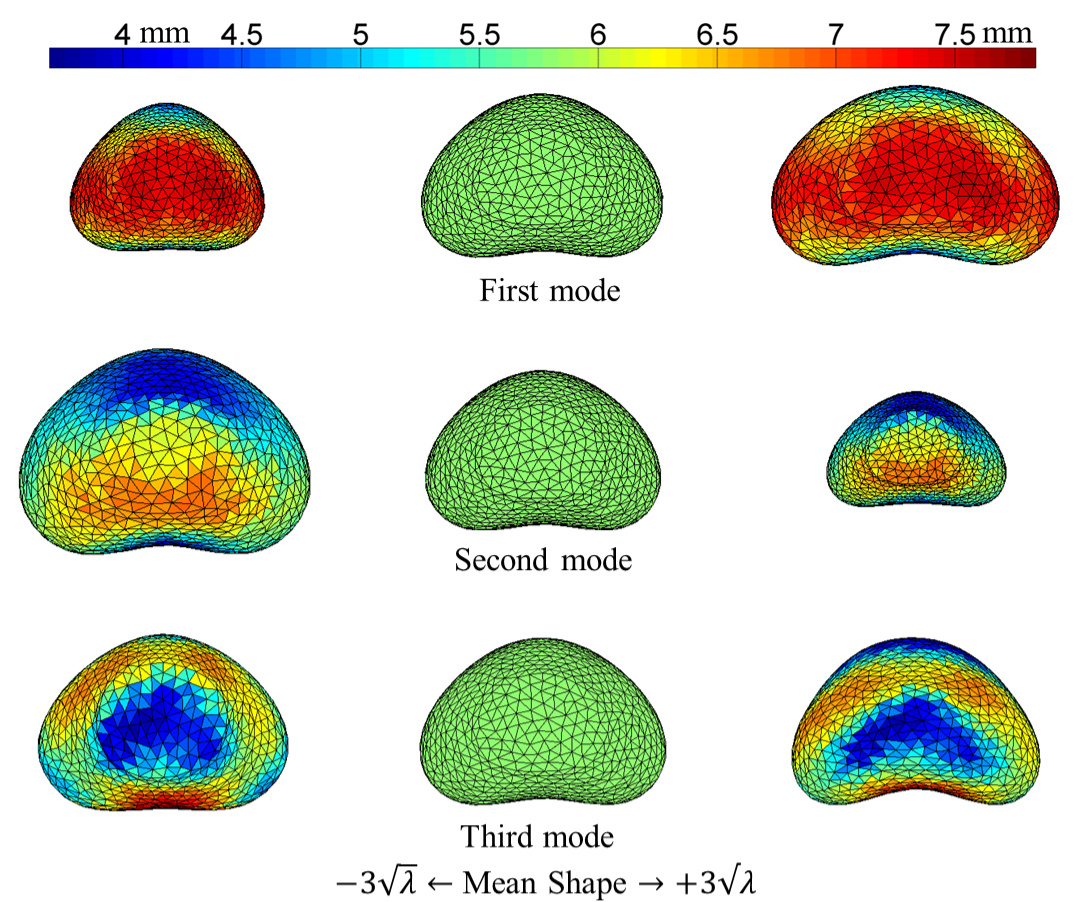
\includegraphics[width=\columnwidth]{images/SSM_modes_inferior}
	\caption{Graphical representation of the prostate shapes described by the SSM after varying weights corresponding to the first three principal modes of variation by three standard deviations ($3\sqrt{\lambda})$. The mean shape is shown with a green model in the middle column. The amount of variation in the left and right column is color coded for each mode.}\label{fig:SSM_modes}
\end{figure}
%%%%%%%%%%%%%%%%%%%%%%%%%%%%%%%%%
%%%%%%%%%%%%%%%%%%%%%%%%%%%%%%%%%%%%%%
\begin{equation} \label{eq:GMMFEM1}
\Gamma\vec{u} = \Upsilon,
\end{equation}
%%%%%%%%%%%%%%%%%%%%%%%%%%%%%%%%%%%%%%
where $P,\sigma^2$ describes a GMM that corresponds to the full source surface and
%%%%%%%%%%%%%%%%%%%%%%%%%%%%%%%%%%%%%%
\begin{eqnarray} \label{eq:GMMFEM2}
 \Gamma &=& \beta \sigma^2K + s^2\trans{\tilde{\Phi}}\diag\left(\tilde{P}1\right)\tilde{\Phi}\\
 \Upsilon &=& s\trans{\tilde{\Phi}}\trans{\tilde{R}}\tilde{P}\vec{x}_\mathrm{target}\nonumber\\
 && -\trans{\tilde{\Phi}}\diag\left(\tilde{P}1\right)\left(s^2\vec{y}_\mathrm{source}+s\tilde{I}\trans{R}t\right)\nonumber.
\end{eqnarray}
%%%%%%%%%%%%%%%%%%%%%%%%%%%%%%%%%%%%%%
\section{Experiments and Results}
%%%%%%%%%%%%%%%%%%%%%%%%%%%%%%%%%
In this section, we evaluate the proposed nonrigid registration method in a series of experiments with MR-TRUS image pairs acquired from patients who underwent a prostate intervention. The data acquisition protocol was approved by the institutional ethics board, and in each case patients provided written consent to be included in the study. The rest of this section is divided into four subsections. In Section~\ref{sec:ssm}, we discuss the training population used for SSM construction. In Section~\ref{sec:biopsy}, we discuss the biopsy data acquisition, segmentation protocol and the initialization of the registration. In Section~\ref{sec:exp1}, we validate the accuracy of our registration method by measuring the TRE between pairs of intrinsic fiducials found in the interior of the prostate. To highlight the importance of the SSM, we compare the outcome of SSM-FEM registration with and without the SSM and FEM components. In Section~\ref{sec:exp2}, we investigate the sensitivity of our approach to missing observations in both full and partial surfaces. Finally, in Section~\ref{sec:exp3}, we investigate the sensitivity of our approach to parameters that control the regularization terms in the registration.
%%%%%%%%%%%%%%%%%%%%%%%%%%%%%%%%%
\subsection{Data}
%%%%%%%%%%%%%%%%%%%%%%%%%%%%%%%%%
\subsubsection{SSM Construction}\label{sec:ssm}
%%%%%%%%%%%%%%%%%%%%%%%%%%%%%%%%%
A suitable choice for training data is a large population of prostate images that are acquired using the same modality. The choice of the imaging modality is important, since biomechanical forces, e.g. end-firing probes and endorectal coils, affect the shape of the prostate in TRUS and MRI, respectively. Ideally, the prostates should be in the same biomechanical deformation state and differences in appearance should be due inter-subject variations. Finally, for surface-based SSMs, the prostate needs to be accurately and reliably segmented.

Brachytherapy volumes are routinely acquired and segmented in large clinics and interventional centers. We used a dataset of 290 brachytherapy patients in the construction of our SSM. Each TRUS volume consists of 7 to 14 parallel equally spaced ($5$~mm apart) axial B-mode images of the prostate which are captured using a side-firing transrectal probe. For each B-mode image, the prostate gland is delineated using a standard of care software, which is based on the semi-automatic prostate segmentation method presented by Mahdavi~\textit{et al.}~\cite{Mahdavi11a}. These contours are manually corrected afterwards by an expert clinician, and subsequently used as the training population in our SSM construction.

As mentioned earlier, we used the group-wise GMM method~\cite{Rasoulian12b} for the construction of the SSM. This resulted in a SSM with a mean shape containing 1000 nodes and 1996 faces. Figure~\ref{fig:SSM_modes} shows the deviation of the instances from the mean using different modes of variation. The first two modes control the scale, whereas the third mode controls the curvature of the prostate.

%%%%%%%%%%%%%%%%%%%%%%%%%%%%%%%%%
\begin{figure}[t]
	\centering
	\subfloat[][Base\label{fig:MRData1}]{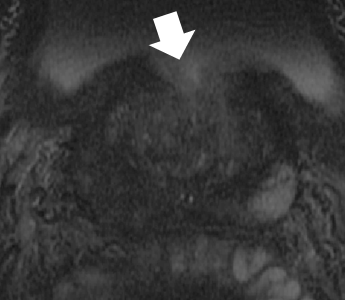
\includegraphics[width=0.33\columnwidth,height=1.2in]{images/MRData1}} \hfill
	\subfloat[][Mid-gland\label{fig:MRData2}]{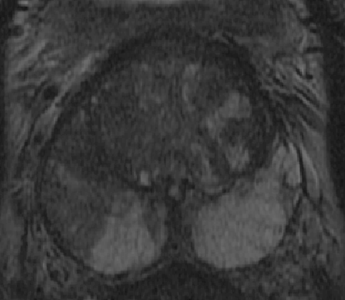
\includegraphics[width=0.33\columnwidth,height=1.2in]{images/MRData2}} \hfill
	\subfloat[][Apex\label{fig:MRData3}]{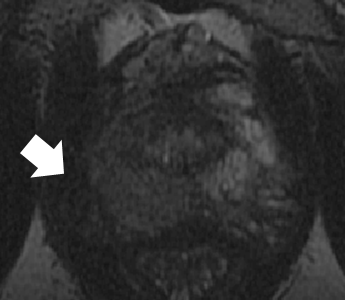
\includegraphics[width=0.33\columnwidth,height=1.2in]{images/MRData3}}\\
	\subfloat[][Base\label{fig:TRUSData1}]{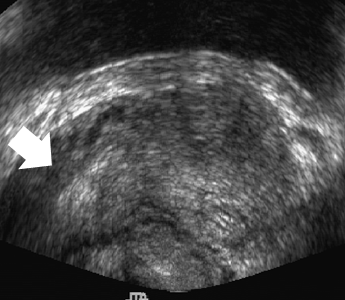
\includegraphics[width=0.33\columnwidth,height=1.2in]{images/USData1}} \hfill
	\subfloat[][Mid-gland\label{fig:TRUSData2}]{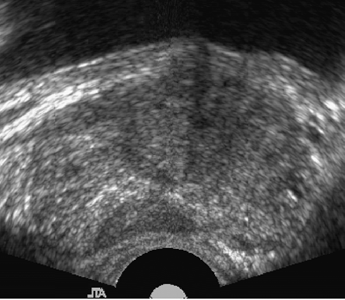
\includegraphics[width=0.33\columnwidth,height=1.2in]{images/USData2}} \hfill
	\subfloat[][Apex\label{fig:TRUSData3}]{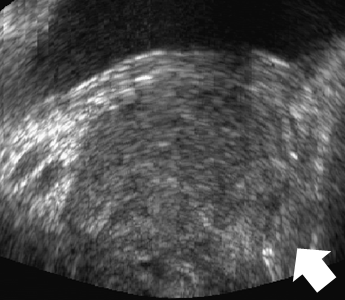
\includegraphics[width=0.33\columnwidth,height=1.2in]{images/USData3}}\\
	\subfloat[][MR Segmentation\label{fig:MRSeg}]{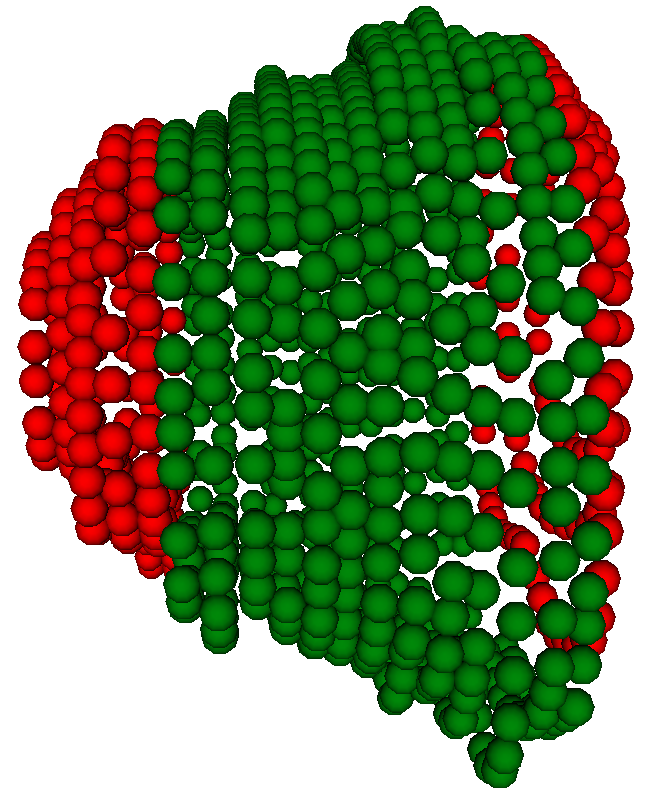
\includegraphics[width=0.33\columnwidth]{images/MR_Segmentation}}\hfill
	\subfloat[][TRUS Segmentation\label{fig:TRUSSeg}]{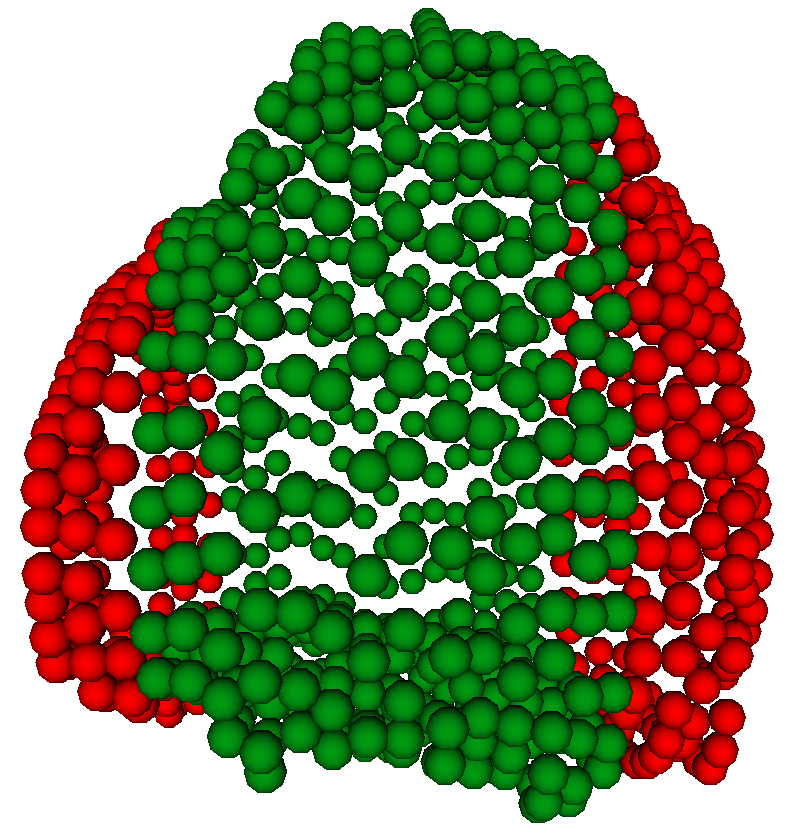
\includegraphics[width=0.33\columnwidth]{images/TRUS_Segmentation}}	
  \caption{Axial slices from MR (top-row) and TRUS (middle-row) volumes. Typically, the prostate boundary can be accurately and reliably segmented in the mid-gland, i.e. (b) and (e). White arrows highlight regions where the true prostate boundary is ambiguous. (g) and (h) depict the resulting segmentation of MR and TRUS, respectively. Partial segmentations are color coded in green, uncertain contours are highlighted in red.}\label{fig:biopsy1}
\end{figure}
%%%%%%%%%%%%%%%%%%%%%%%%%%%%%%%%%

The choice of the number of modes is governed by the compactness of the resulting SSM. Compactness simply measures the accumulative variance of the model~\cite{Heimann09a}. A popular rule of thumb is the first $L$ modes that span 95\% of the total modes of variation. For our SSM, this results in a model with 50 principal modes of variation.
%%%%%%%%%%%%%%%%%%%%%%%%%%%%%%%%%
\subsubsection{Prostate Biopsy}\label{sec:biopsy}
%%%%%%%%%%%%%%%%%%%%%%%%%%%%%%%%%
The validation data was acquired from ten patients scheduled for prostate biopsy. Figure~\ref{fig:biopsy1} shows typical MR and TRUS images acquired from a patient. The T2-weighted MR images were acquired using a 3 Tesla GE Excite HD MRI system (Milwaukee, WI, USA) with a spacing of $0.27~\times~0.27~\times~2.2$ mm. Typical slices from base, mid-gland and apex are shown in Figures~\ref{fig:MRData1},\ref{fig:MRData2} and \ref{fig:MRData3}, respectively. The TRUS images were acquired using a 3D-TRUS mechanical biopsy system~\cite{Bax08a} with a Philips HDI-5000 US machine and a C9-5 transducer using an axial rotation of the biopsy probe. The TRUS images were reconstructed into a 3D-volume with a spacing of $0.19~\times~0.19~\times~0.19$ mm. Figures~\ref{fig:TRUSData1},\ref{fig:TRUSData2} and \ref{fig:TRUSData3} show typical slices from base, mid-gland and apex, respectively. In each modality, areas around the mid-gland, e.g. Figures~\ref{fig:MRData2} and \ref{fig:TRUSData2}, where the prostate boundary could be reliably and accurately traced, were segmented. We refer to these contours as \textbf{partial} segmentation. Additionally, we segmented regions of the prostate were the prostate boundary was not easily visible, i.e. base and apex, using symmetry and the general ellipsoid shape of the prostate. The white arrows in Figure~\ref{fig:biopsy1} are examples of these uncertain regions. The prostate contours extracted from these uncertain regions are referred to as \textbf{uncertain data}. The combination of uncertain and partial data is referred to as \textbf{full data}. An example segmentation of MR and TRUS is shown in Figures~\ref{fig:MRSeg} and \ref{fig:TRUSSeg}, respectively. To initialize the registration, the full prostate surfaces from the MRI and TRUS are brought to an initial position with respect to the mean shape using right-anterior-superior (RAS) coordinates and center of mass alignment.
%%%%%%%%%%%%%%%%%%%%%%%%%%%%%%%%%
\subsection{Registration of Full and Partial Surfaces}\label{sec:exp1}
%%%%%%%%%%%%%%%%%%%%%%%%%%%%%%%%%
\begin{figure}[t]
	\centering
	\subfloat[][Initial\label{fig:InitFull}]{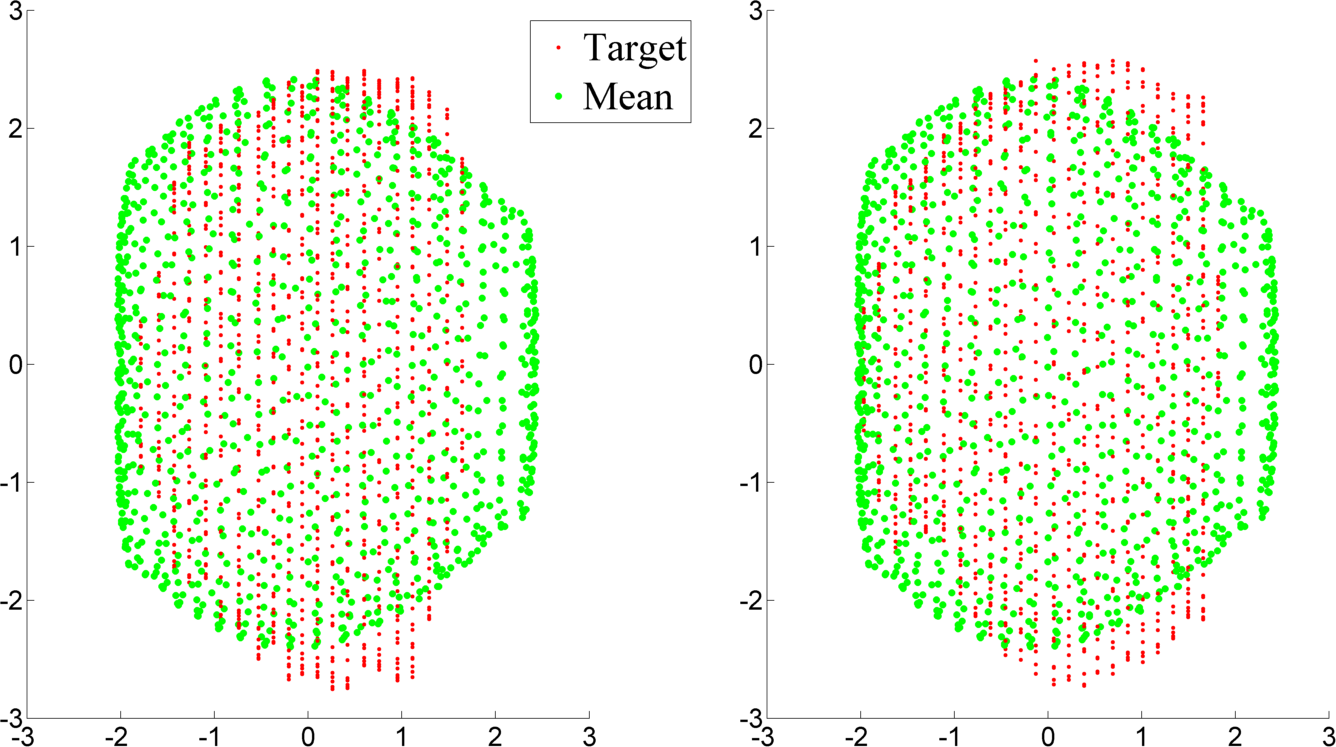
\includegraphics[width=\columnwidth]{images/SSM_FEM_Full_Initial}}\\
	\subfloat[][Registered\label{fig:Resultfull}]{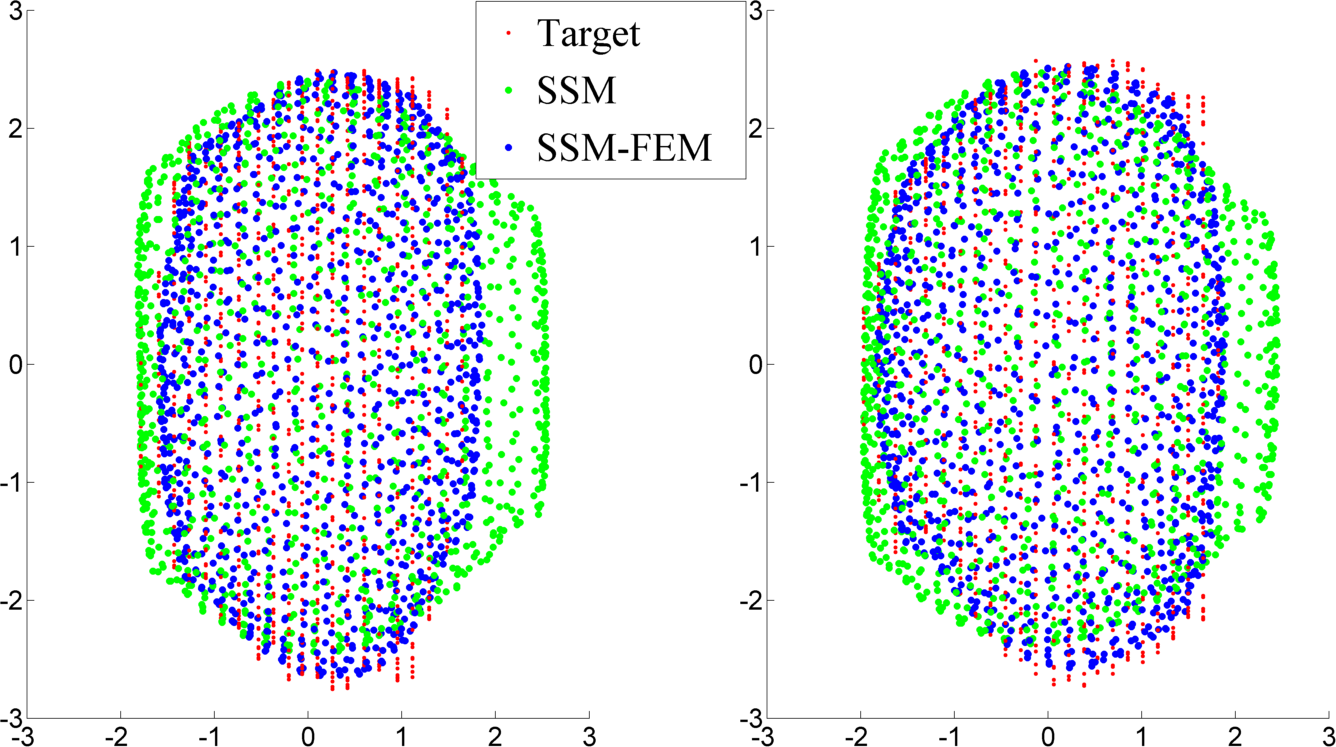
\includegraphics[width=\columnwidth]{images/SSM_FEM_Full_Registered}}
	\caption{An example of SSM-FEM registration with $w=0.0$, $\mu=400$, $\beta=10.0$, $E=5.0$~kPa and $\nu=0.49$ to full data. Following center of mass initialization (a), the SSM mean is evolved to target surfaces (b). The target surfaces are shown in red, the current instance is shown in green and the result of SSM-FEM registration is shown in blue.}\label{fig:RegFull}
\end{figure}
%%%%%%%%%%%%%%%%%%%%%%%%%%%%%%%%%
%%%%%%%%%%%%%%%%%%%%%%%%%%%%%%%%%
\begin{figure}[t]
	\centering
	\subfloat[][Initial\label{fig:InitPartial}]{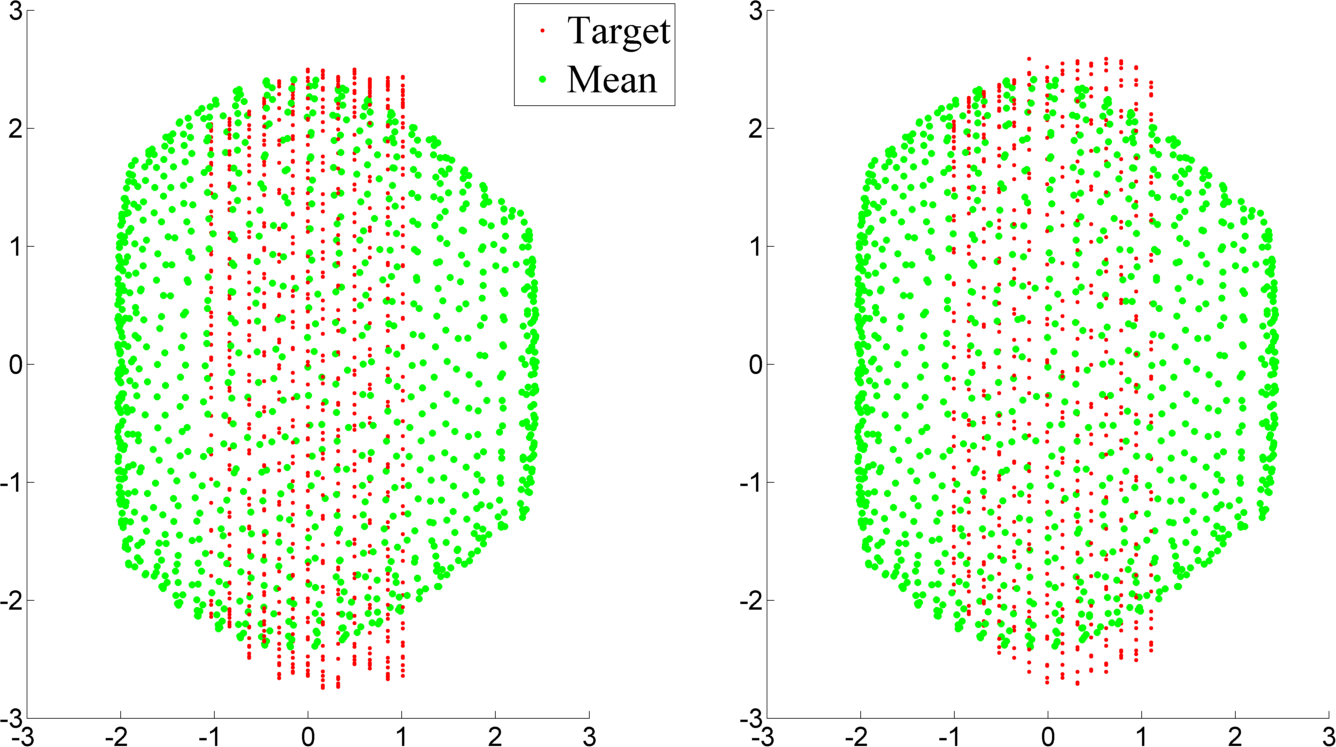
\includegraphics[width=\columnwidth]{images/SSM_FEM_Partial_Initial}}\\
	\subfloat[][Registered\label{fig:ResultPartial}]{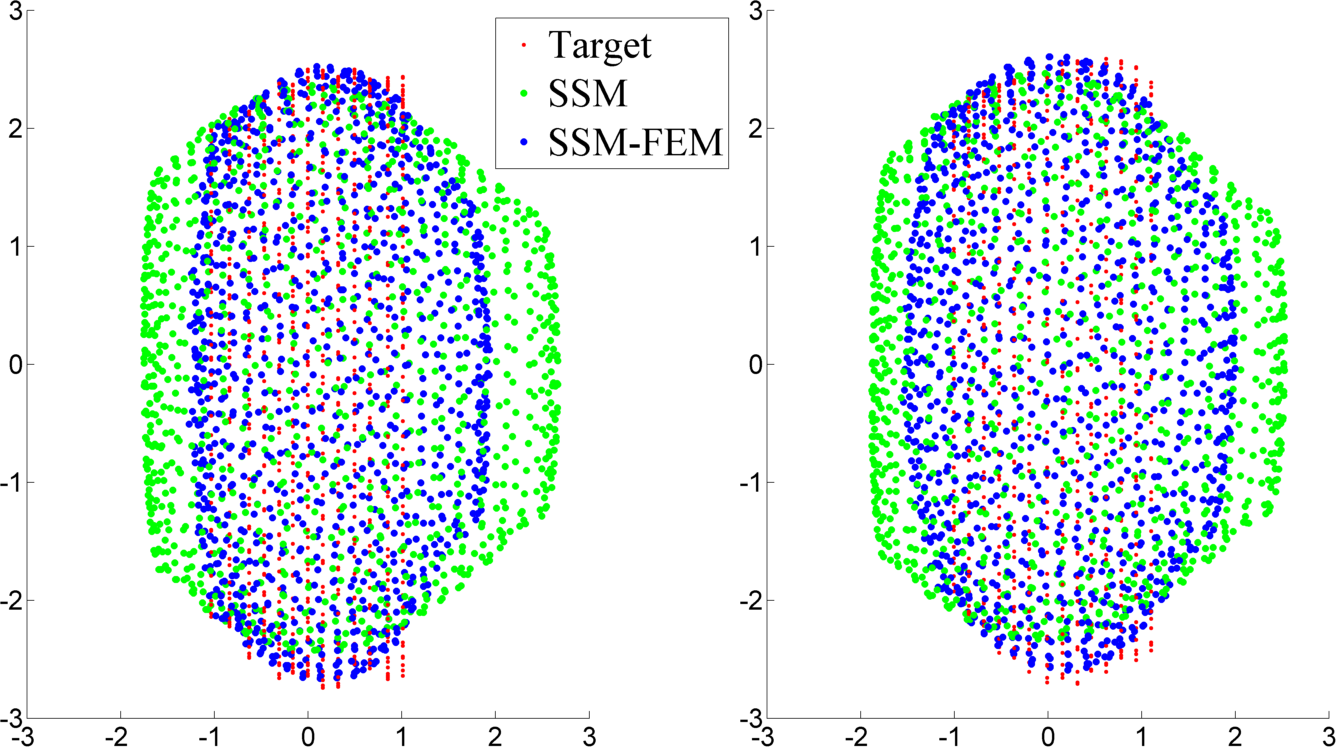
\includegraphics[width=\columnwidth]{images/SSM_FEM_Partial_Registered}}
	\caption{An example of SSM-FEM registration with $w=0.2$, $\mu=400$, $\beta=10.0$, $E=5.0$~kPa and $\nu=0.49$ to partial data. Following center of mass initialization (a), the SSM mean is evolved to target surfaces (b). The target surfaces are shown in red, the current instance is shown in green and the result of SSM-FEM registration is shown in blue.}\label{fig:RegPartial}
\end{figure}
%%%%%%%%%%%%%%%%%%%%%%%%%%%%%%%%%
As a first set of experiments, we used the biopsy data described in Section~\ref{sec:biopsy} to validate our registration pipeline on full and partial surfaces. Following center of mass initialization between the SSM-mean and target surfaces, as seen in Figure~\ref{fig:InitFull}, a typical SSM-FEM registration result to a full MR-TRUS surface pair is shown in Figure~\ref{fig:Resultfull}. The Tikhonov and biomechanical regularization weights were tuned such that the best surface overlap was achieved. This resulted in a choice of $\mu=400$ and $\beta=10$,  respectively. Since full surfaces do not have any missing points, we set the estimate of missing data, $w_\mathrm{md}$, to zero throughout this experiment. To maintain a fair comparison, we used the same parameters for SSM and GMM-FEM registration methods as well.

For partial surfaces, we performed a similar experiment. Following center of mass initialization in Figure~\ref{fig:InitPartial}, a typical SSM-FEM registration result to a partial MR-TRUS surface pair is shown in Figure~\ref{fig:ResultPartial}. We used the same Tikhonov and biomechanical regularization weights as full data. However, since partial surfaces exhibit missing points, we set the estimate of missing data, $w_\mathrm{md}$, to $0.2$ throughout this experiment. To maintain a fair comparison, the same parameters were used for SSM and GMM-FEM registration methods.
%%%%%%%%%%%%%%%%%%%%%%%%%%%%%%%%%
\subsubsection{Quantitative Validation}
%%%%%%%%%%%%%%%%%%%%%%%%%%%%%%%%%
\begin{figure}[t]
	\centering
	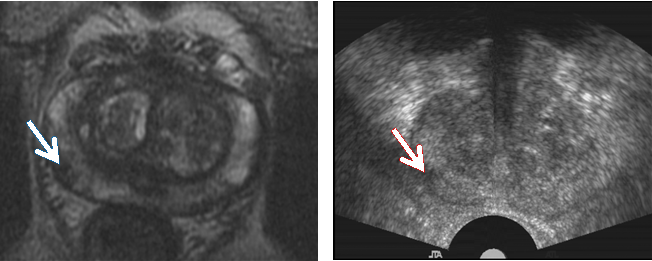
\includegraphics[width=\columnwidth]{images/FiducialPair}
	\caption{Examples of fiducial pairs in MR (left) and TRUS (right) images.}\label{fig:Fiducial}
\end{figure}
%%%%%%%%%%%%%%%%%%%%%%%%%%%%%%%%%
Our algorithm was implemented in Matlab (MathWorks, MA), and converges within $\approx30$~seconds on a $3.4$~GHz Intel Core i7 CPU with $8.00$~GB of RAM. In order to quantify the registration results, we asked an expert radiologist to select five intrinsic fiducials per patient consisting of cysts and benign prostatic hyperplasia (BPH). Figure~\ref{fig:Fiducial} shows an example of corresponding fiducial pairs in MR and TRUS. The $L_2$ distance between these fiducial pairs was used to quantify the TRE.

The mean and standard deviation of the TRE and its $p$-value are shown in Tables~\ref{tab:TRE} for full and partial data. For full surfaces, SSM, GMM-FEM and SSM-FEM methods decrease the TRE following registration. The mean TRE for SSM, GMM-FEM and SSM-FEM registration methods is decreased by $0.79$~mm, $1.88$~mm and $1.95$, respectively. The mean TRE for SSM-FEM registration is $1.16$~mm lower compared to SSM registration. This result suggests that the transformation between MR and TRUS surfaces is not rigid and nonrigid deformations exist. 

For partial surfaces, SSM and SSM-FEM registration methods decrease the TRE by $0.64$~mm and $1.78$, respectively. However, following GMM-FEM registration, the TRE is increased by $0.32$~mm. Upon inspection, we observed that the increased error is due to convergence to a local minima, where a mirroring of partial surfaces resulted in a smaller value in the objective functional. This result suggests that the SSM component of the proposed registration method is required when both surfaces are only partially segmented.

In order to investigate the statistical significance of the registration results, we first investigated if the TRE distributions were normal. Using a one-sample Kolmogorov-Smirnov test, the TREs were found not to be normally distributed at the 95\% significance level ($p<1e-4$). As a result, we performed a set of Wilcoxon signed-rank tests on the TREs. The null hypothesis is that the TREs of the initialization and the subsequent registration method share a common median at the 95\% significance level. The p-values are also reported in Table~\ref{tab:TRE}. These results show the differences in the TREs are statistically significant. 

Finally, in order to investigate the statistical significance of the proposed registration algorithm over other nonrigid methods used for comparison, we performed two additional Wilcoxon signed-rank tests. The first is performed between SSM-FEM and SSM. The signed-rank test shows the improvement for GMM-FEM is statistically significant ($p\leq1e-6$). The second signed-rank test is between SSM-FEM and GMM-FEM. Although the TRE is reduced, the signed-rank test fails to reject the null hypothesis for prostatectomy data. This implies that the improvement of SSM-FEM based registration over GMM-FEM is not significant for full surfaces. However, for partial surfaces, the signed-rank test shows that the improvement is statistically significant for SSM-FEM over GMM-FEM ($p\leq1e-4$). This result suggests that the SSM-FEM does outperform GMM-FEM when both surfaces are only partially segmented.
%%%%%%%%%%%%%%%%%%%%%%%%%%%%%%%%%
\begin{table}[tb]
\begin{center}
\caption{Mean and standard deviation of the TRE (mm) following initial alignment and after SSM, GMM-FEM and SSM-FEM registration on full and partial surfaces. The $p$-values show the result of Wilcoxon signed-rank tests between initially aligned surfaces and subsequent registration methods.}
\centering
\begin{tabular}{c| c| c| c| c}
	\hline
	& \multicolumn{2}{c|}{TRE} & \multicolumn{2}{c}{$p$-value}\\
	\cline{2-3}  \cline{4-5}
	Method & Full & Partial & Full & Partial \\
	\hline
	Initial & $4.51 \pm 1.21$ & $4.73 \pm 1.31$ & NA & NA \\
	\hline
	SSM & $3.72 \pm 1.17$ & $4.09 \pm 1.63$ & $1e-2$ & $0.33$ \\
	\hline
	GMM-FEM & $2.63 \pm 1.05$ & $5.05 \pm 1.56$ & $1e-3$ & $0.27$ \\
	\hline
	SSM-FEM & $2.56 \pm 0.93$ & $2.95 \pm 0.55$ & $1e-4$ & $1e-4$ \\
   \hline
\end{tabular}
\label{tab:TRE}
\end{center}
\end{table}
%%%%%%%%%%%%%%%%%%%%%%%%%%%%%%%%%
\begin{figure}[t]
	\centering
	\subfloat[][Box-plot distribution of robustness as observations are removed\label{fig:MissingBox}]{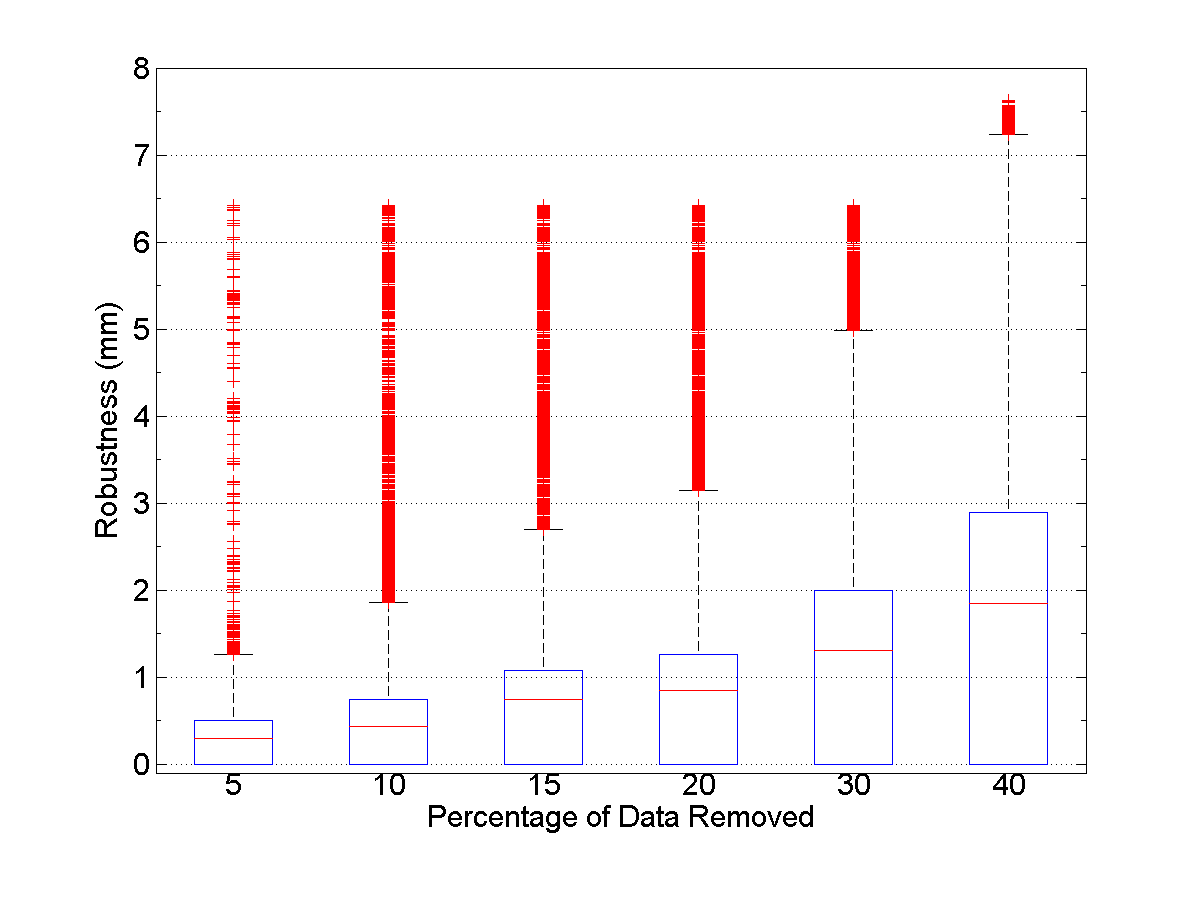
\includegraphics[width=\columnwidth]{images/MissingDataBar}}\\
	\subfloat[][Left to right: Spatial distribution of robustness for SSM-FEM registration when 10\%, 20\% and 40\% of observations are removed.\label{fig:MissingSpatial}]{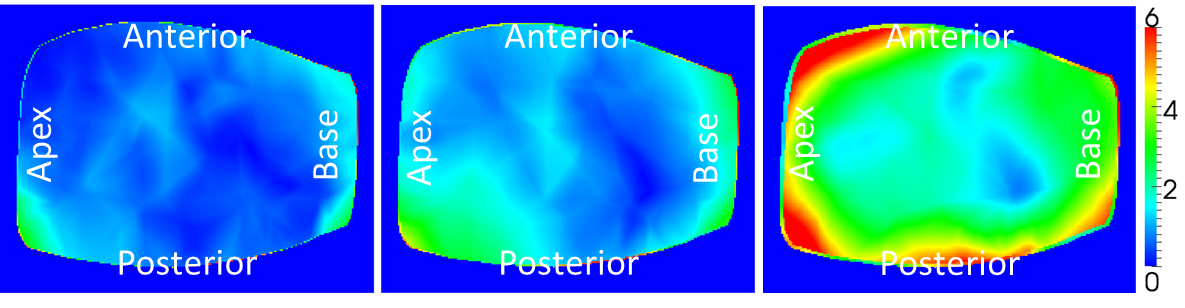
\includegraphics[width=\columnwidth]{images/MissingDataSpatial}}
	\caption{Distribution of robustness as different percentages of observations are removed with $E=5.0$~kPa, $\mu=400$, $\beta=10.0$, and $\nu=0.49$. Sagittal slice of robustness for SSMM-FEM registration when different amounts of observations are removed. For better visualization, distances larger than 6~mm are shown in the same color.}\label{fig:Missing}
\end{figure}
%%%%%%%%%%%%%%%%%%%%%%%%%%%%%%%%%
\subsection{Sensitivity to Missing Surface Points}\label{sec:exp2}
%%%%%%%%%%%%%%%%%%%%%%%%%%%%%%%%%
%%%%%%%%%%%%%%%%%%%%%%%%%%%%%%%%%
\begin{figure*}[t]
	\centering
	\subfloat[][Box-plot distribution of robustness as $\beta$ is perturbed\label{fig:BetaBox}]{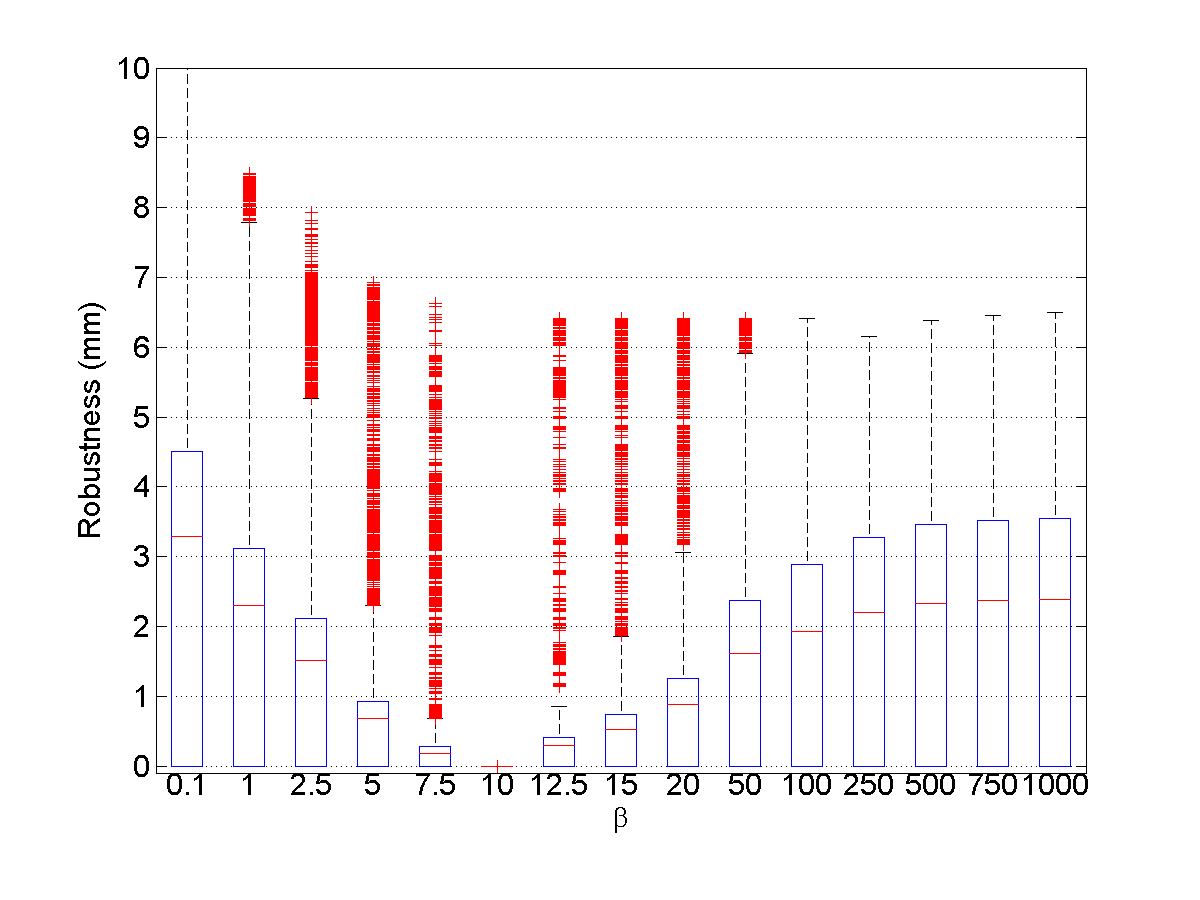
\includegraphics[width=\columnwidth]{images/Boxplot_beta}}\hfill
	\subfloat[][Box-plot distribution of robustness as $\mu$ is perturbed\label{fig:MuBox}]{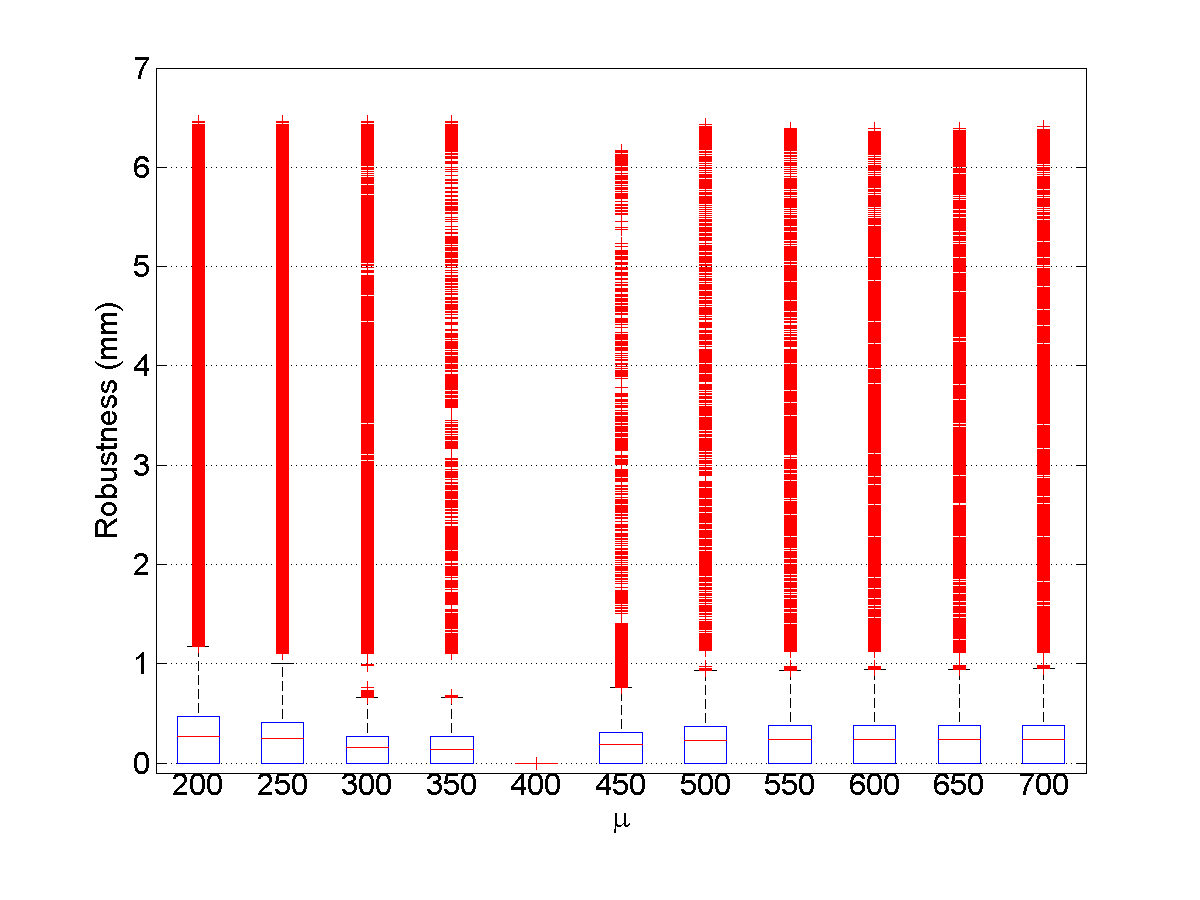
\includegraphics[width=\columnwidth]{images/Boxplot_mu}}\\
	\subfloat[][Left to right: Spatial distribution of robustness for SSM-FEM registration when $\beta$ is set to 2.5, 7.5 and 20.0, respectively.\label{fig:BetaSpatial}]{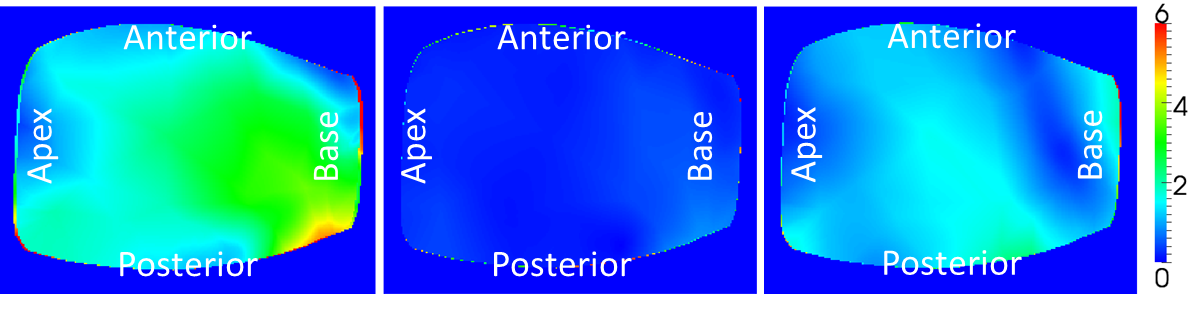
\includegraphics[width=\columnwidth]{images/BetaSpatial}}\hfill
	\subfloat[][Left to right: Spatial distribution of robustness for SSM-FEM registration when $\mu$ is set to 200, 350 and 550, respectively.\label{fig:MuSpatial}]{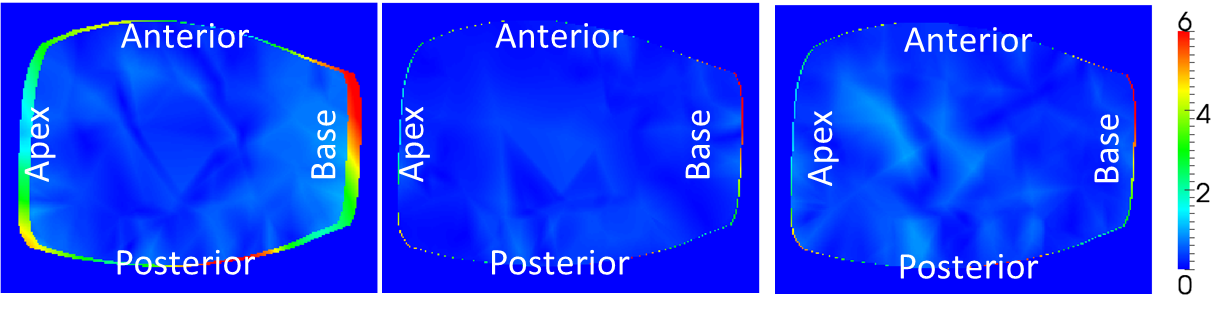
\includegraphics[width=\columnwidth]{images/MuSpatial}}
	\caption{Robustness of SSM-FEM registration for different biomechanical (a) and Tikhonov regularization weights (b). Biomechanical parameters are perturbed around parameters which provided the best surface overlap ($E=5.0$~kPa, $\nu=0.49$, $\mu=400$ and $\beta=10.0$). For better visualization, distances larger than 6~mm are shown with the same color.}\label{fig:Perturb}
\end{figure*}
%%%%%%%%%%%%%%%%%%%%%%%%%%%%%%%%%
In the second set of experiments, we investigate the robustness of our method when parts of the observations were missing. This provides a measure of confidence of the TRE in regions where the prostate is not segmented. Robustness is defined as the performance of an algorithm in the presence of disruptive factors~\cite{Jannin02a}. To this end, we systematically removed portions of observation points (i.e. rows of $X_\mathrm{md}$) from both the base and apex (from 2.5\% to 20\% from each). Subsequently, we applied our algorithm to the cropped observations. No points were removed from the SSM surface (i.e rows of $Z$), since we assume that the SSM can be reliably and accurately constructed. In order to quantify the performance, we compared the internal deformation fields with and without missing observations from the MR coordinate space to the TRUS space. We explicitly define robustness as the $L_2$ distance of the deformation field computed with missing observations to the deformation field computed when no observations are removed. This implicitly defines robustness as the fidelity of the registration in recovering the same deformation field without missing data, i.e. a smaller value corresponds to a better robustness. 

The results of this experiment are shown in Figure~\ref{fig:Missing} for a typical biopsy patient. Excluding outliers in Figure~\ref{fig:MissingBox}, internal deformations stay below $2.0$~mm when $10\%$ of the observations are removed from the SSM-FEM registration. The robustness of SSM-FEM registration progressively declines as more observations in the base and apex regions are removed. As seen in Figure~\ref{fig:MissingSpatial} The deformation field in the central region of the prostate seems more robust to missing data compared to base and apex regions. One possible explanation is that nodes interior to the prostate are constrained by more adjacent nodes compared to surface nodes near the base and apex where data is removed.
%%%%%%%%%%%%%%%%%%%%%%%%%%%%%%%%%
\subsection{Sensitivity to Regularization Parameters}\label{sec:exp3}
%%%%%%%%%%%%%%%%%%%%%%%%%%%%%%%%%
In the final set of experiments, we investigate robustness of our method to parameters that control the regularizers. Specifically, we investigate the effect of changing the Tikhonov and biomechanical regularization weights, i.e. $\mu$ and $\beta$, on the composition of the MR-TRUS deformation field. We recommend a value of $\nu=0.49$ for Poisson's ratio, since we assume the prostate to maintain a constant volume. We do not investigate the effect of changing the Young's modulus since, under the assumption of homogeneous elasticity, it can be shown that the stiffness matrix has a linear relationship with this values. As a result, the only two free parameters for the proposed registration algorithm are $\mu$ and $\beta$. In order to examine the sensitivity of our registration method to these parameters, we perturbed the values for these regularization weights, which is shown in Figure~\ref{fig:Perturb}.

As seen in Figure~\ref{fig:BetaBox}, the SSM-FEM registration can be sensitive to the biomechanical regularization weight. When tuning this parameter, the registration approach exhibited three distinct behaviors. For large regularization weights, in this case $\beta\geq50.0$, the FEM behaved similar to a rigid object. For very small regularization weights, in this case $\beta\leq2.5$, the FEM does not provide any regularization and the surface is allowed to move independently of interior nodes. Finally, for regularization values in between two extremes, the registration is constrained using the biomechanical properties of the tissue.  This parameter should be tuned to trade-off between surface-fitting and internal deformation.

Figure~\ref{fig:BetaSpatial} shows the spatial distribution of robustness for three different behaviors described above. The deformation field around the mid-gland seems less robust to perturbations in the regularization weight compared to base and apex. One possible explanation is that the prostate shape is much different due to probe-induced biomechanical forces.

Figure~\ref{fig:MuBox} shows the sensitivity of the internal deformation field to Tikhonov weight. The registration seems less sensitive to perturbations in this parameter compared to the biomechanical regularization weight. For small Tikhonov values, $\mu\leq200.0$, due to the different appearance of the prostate in MR and TRUS surfaces, the registration becomes unstable, and Equation~\ref{eq:SSM1} produces invalid instances. For large Tikhonov values, $\mu\geq550.0$, the SSM is restricted to instances close to the mean shape. For values between these two extremes, the search space of the registration is restricted to valid instances of the SSM. As seen in Figure~\ref{fig:MuSpatial}, changes in the Tikhnov weight mostly affect the boundary of the prostate, and regions inside the prostate seem less sensitive to perturbations in this parameter.
%%%%%%%%%%%%%%%%%%%%%%%%%%%%%%%%%
\section{Discussion and Conclusions}
%%%%%%%%%%%%%%%%%%%%%%%%%%%%%%%%%
In this paper, we presented a novel nonrigid surface-based registration approach that is robust to missing data. The proposed registration algorithm converges within thirty seconds on a regular desktop PC. We showed the internal deformation found through our proposed method to be robust up to $2.0$~mm when 10\% of observations are removed. A great advantage of the algorithm is that it estimates point-correspondences, nodal displacements, shape and pose parameters in a single minimization step.  This is one of the contributing factors to the efficiency of the algorithm.  We also obtain a full volumetric deformation field for the object of interest as a by-product of the regularization, whereas in many existing surface-based approaches, volumetric deformation needs to be estimated with an additional post-processing step.

The most time-consuming portion of the registration method is the FE meshing component, which is called every time a new instance is generated. If further speed-up is necessary, it is possible to perform meshing only when the generated instance differs significantly from the previous iteration. Another shortcoming of our algorithm is that it requires the MR and TRUS to be segmented prior to the registration. While the MR can be segmented days ahead of time, the 3D-TRUS needs to be segmented within minutes due to clinical requirements. One possible solution is to use an existing fast segmentation method~\cite{Qiu12a}. Of course, since the method is designed to be extremely robust to missing data, we suggest to only segment regions in which the boundary of the anatomy can be clearly distinguished, such as in the mid-gland. This can also help speed up the segmentation process.

In Section~\ref{sec:exp1} we investigated the performance of our registration method using fiducial pairs found in the interior of the prostate. The SSM-FEM algorithm yields a statistically significant improvement following registration ($1.8$~mm). While the improvement is small, it should be compared to the acceptable error bounds of a targeted biopsy system. With a TRE of $2.5$~mm, one can obtain a confidence interval corresponding to two standard deviations from the mean, i.e. the estimated true center of the tumor. If this requirement is met, then 95\% of registered targets come within the clinically significant $5$~mm radius~\cite{Karnik10a}. Our improvement on TRE brings us closer to the acceptable error bounds of a targeted biopsy system.

In this manuscript, we used an isotropic GMM to model surface nodes on the SSM and used the EM framework to estimate the correspondences between SSM and TRUS/MR surfaces. While isotropic GMMs have been shown to be effective in rejecting noise/outliers~\cite{Myronenko10a}, this assumption breaks in the presence of anisotropic noise. To tackle this issue, similar to Zheng~\cite{Zheng13a}, the proposed method can be easily extended to include anisotropic GMMs in an expectation conditional maximization (ECM) framework~\cite{Horaud11a}.

While the set of observations in this manuscript was limited to the boundary of the prostate extracted from two modalities, the proposed registration method can easily be extended to concurrently register more than two surfaces. Such a situation may arise when the patient is scheduled for a re-biopsy, and it is desirable to simultaneously register MR, the previous and current TRUS surfaces. This would enable the radiologist to avoid areas that in the previous biopsy were found to be cancer-free and enable re-sampling areas that are prone to develop cancer, such as BPH and suspicious MR regions.

In this paper, we used a linear, homogeneous material to create the prostate finite element model. However for most soft tissue, some degree viscoleastic, poroelastic, anisotropic and nonlinear response is expected when a mechanical force is applied. If the nonlinear response is significant, non-linear models, such as Mooney-Rivlin, can easily be included by linearizing about the current deformation state and updating the stiffness matrix at each iteration. This will introduce an additional synthetic force to be added to the objective function that encodes the current state. As for the tissue elastic modulus, the scope of the current manuscript is limited to homogeneous materials and its extension to inhomogeneous materials is not straightforward. If additional elastic information about the elastic properties of the tissue is available, probably through real-time elastography, then a back-projection of elastic values to the space of the instance is required. This is one possible extension of this work.
%%%%%%%%%%%%%%%%%%%%%%%%%%%%%%%%%
\section*{Acknowledgements}
%%%%%%%%%%%%%%%%%%%%%%%%%%%%%%%%%
This work was supported by the Natural Sciences and Engineering Research Council of Canada (NSERC) and the Canadian Institutes of Health Research (CIHR).
%%%%%%%%%%%%%%%%%%%%%%%%%%%%%%%%%
\appendices
%%%%%%%%%%%%%%%%%%%%%%%%%%%%%%%%%
\section{Derivation of FE Nodal Displacements}\label{sec:app1}
%%%%%%%%%%%%%%%%%%%%%%%%%%%%%%%%%
Minimization of Equation~\ref{eq:objTotal2} w.r.t. nodal displacements in each modality is equivalent to the registration of an instance of the SSM to one sets of observations. To avoid clutter, we drop the modality subscript, $\mathrm{md}$, throughout this section.

Ignoring terms independent of $U$, Equation~\ref{eq:objMod2} is written as:
%%%%%%%%%%%%%%%%%%%%%%%%%%%%%%%%%
\begin{align}\label{eq:FE1}
  \mathcal{E}(U) & = \dfrac{1}{2\sigma^2}\sum_{m,n=1}^{M,N}P(z_m|x_n)\left\|x_n-sR\left(y_m+\Phi_mU\right)-t\right\|^2\notag\\
  & + \dfrac{\beta}{2}\trans{\vec{u}}K\vec{u},
\end{align}
%%%%%%%%%%%%%%%%%%%%%%%%%%%%%%%%%
where $\vec{u}=\trans{(u_{11},\ldots,u_{1D},\ldots,u_{JD})}$ is the rasterized representation of $U$. We can rewrite Equation~\ref{eq:FE1} in matrix form:
%%%%%%%%%%%%%%%%%%%%%%%%%%%%%%%%%
\begin{align}\label{eq:FE2}
    \mathcal{E}(U) & = \dfrac{1}{2\sigma^2}\left[N_P\trans{t}t + \trace\left(\trans{X}\diag\left(\trans{P}1\right)X\right)-2\trans{t}\trans{X}\trans{P}1\right.\notag\\
    & \qquad +s^2\;\trace\left(\trans{(Y+\Phi U)}\diag\left(P1\right)(Y+\Phi U)\right) \notag\\
    & \qquad + 2s\;\trans{t}R\trans{(Y+ \Phi U)}P1\notag\\
    & \qquad \left.-2s\;\trace\left(\trans{X}\trans{P}(Y+\Phi U)\trans{R}\right)\right]\notag\\
    & \qquad + \dfrac{\beta}{2}\trans{\vec{u}}K\vec{u},
\end{align}
%%%%%%%%%%%%%%%%%%%%%%%%%%%%%%%%%
where $\trace(\cdot)$ denotes the trace of a square matrix. To simplify the derivation, we can write the fitting term in Equation~\ref{eq:FE2} in rasterized form such that
%%%%%%%%%%%%%%%%%%%%%%%%%%%%%%%%%
\begin{align}\label{eq:FE3}
    \mathcal{E}(\vec{u}) & = \dfrac{1}{2\sigma^2}\left[N_P\trans{t}t + \trans{\vec{x}}\diag\left(\trans{\tilde{P}}1\right)\vec{x}-2\trans{t}\trans{\hat{I}}\diag\left(\trans{\tilde{P}}1\right)\vec{x}\right.\notag\\
    & \qquad\qquad + s^2\;\trans{(\vec{y}+\tilde{\Phi}\vec{u})}\diag\left(\tilde{P}1\right)(\vec{y}+\tilde{\Phi}\vec{u})\notag\\
    & \qquad\qquad +2s\;\trans{t}R\trans{\tilde{I}}\diag\left(\tilde{P}1\right)(\vec{y}+\tilde{\Phi}\vec{u})\notag\\
    & \qquad\qquad \left.-2s\;\trans{\vec{x}}\trans{\tilde{P}}\tilde{R}(\vec{y}+\tilde{\Phi}\vec{u})\right] + \dfrac{\beta}{2}\trans{\vec{u}}K\vec{u},
\end{align}
%%%%%%%%%%%%%%%%%%%%%%%%%%%%%%%%%
where $\trans{\hat{I}} = \begin{bmatrix} I_{D\times D} & \cdots & I_{D\times D} \end{bmatrix}_{D\times ND}$. Excluding terms independent of $\vec{u}$, Equation~\ref{eq:FE3} can be written as:
%%%%%%%%%%%%%%%%%%%%%%%%%%%%%%%%%
\begin{align}\label{eq:FE4}
    \mathcal{E}(\vec{u}) & = \dfrac{s^2}{2\sigma^2}\trans{\vec{u}}\trans{\tilde{\Phi}}\diag\left(\tilde{P}1\right)\tilde{\Phi}\vec{u} + \dfrac{\beta}{2}\trans{\vec{u}}K\vec{u}\\
    & \quad + \dfrac{1}{\sigma^2}\left[\left(s^2\trans{\vec{y}}+s\;\trans{t}R\trans{\tilde{I}}\right)
        \diag\left(\tilde{P}1\right)-s\;\trans{\vec{x}}\trans{\tilde{P}}\tilde{R}\right]\tilde{\Phi}\vec{u}\notag
\end{align}
%%%%%%%%%%%%%%%%%%%%%%%%%%%%%%%%%
Differentiating with respect to $\vec{u}$ results in:
%%%%%%%%%%%%%%%%%%%%%%%%%%%%%%%%%
\begin{align}\label{eq:FE5}
    \di{\mathcal{E}(\vec{u})}{\vec{u}} & = \left[\dfrac{s^2}{\sigma^2}\trans{\tilde{\Phi}}\diag\left(\tilde{P}1\right)\tilde{\Phi} + \beta K\right]\vec{u}\\
        & \quad + \dfrac{1}{\sigma^2}\left[\trans{\tilde{\Phi}}\diag\left(\tilde{P}1\right)\left(s^2\vec{y}+s\tilde{I}\trans{R}t\right)
        -s\trans{\tilde{\Phi}}\trans{\tilde{R}}\tilde{P}\vec{x}\right].\notag
\end{align}
%%%%%%%%%%%%%%%%%%%%%%%%%%%%%%%%%
Setting Equation~\ref{eq:FE5} equal to zero results in the following set of linear equations:
%%%%%%%%%%%%%%%%%%%%%%%%%%%%%%%%%
\begin{align}\label{eq:FE6}
    \Gamma_\mathrm{FEM}\vec{u} &= \Upsilon_\mathrm{FEM},
\end{align}
%%%%%%%%%%%%%%%%%%%%%%%%%%%%%%%%%
where
%%%%%%%%%%%%%%%%%%%%%%%%%%%%%%%%%
\begin{align}\label{eq:FE7}
\Gamma_\mathrm{FEM} &= \beta \sigma^2K + s^2\trans{\tilde{\Phi}}\diag\left(\tilde{P}1\right)\tilde{\Phi}\\
    \Upsilon_\mathrm{FEM} &= s\trans{\tilde{\Phi}}\trans{\tilde{R}}\tilde{P}\vec{x} - \trans{\tilde{\Phi}}\diag\left(\tilde{P}1\right)\left(s^2\vec{y}+s\tilde{I}\trans{R}t\right).\notag
\end{align}
%%%%%%%%%%%%%%%%%%%%%%%%%%%%%%%%%
\section{Derivation of Shape Parameters}\label{sec:app2}
%%%%%%%%%%%%%%%%%%%%%%%%%%%%%%%%%
In this section we minimize Equation~\ref{eq:objTotal2} w.r.t. shape parameters conditioned by observations in both modalities. Ignoring terms independent of $b$, we can write this equation as:
%%%%%%%%%%%%%%%%%%%%%%%%%%%%%%%%%
\begin{align}\label{eq:SSMD1}
  \mathcal{E}(b) & = \sum_\mathrm{md}\dfrac{1}{2\sigma^2_\mathrm{md}}\sum_{m,n=1}^{M,N_\mathrm{md}}P_\mathrm{md}\left\|x^\mathrm{md}_n-sR\left(z^\mathrm{md}_m+\Psi_mb\right)-t\right\|^2\notag\\
  & + \frac{\mu}{2}\trans{b}\Lambda{b},
\end{align}
%%%%%%%%%%%%%%%%%%%%%%%%%%%%%%%%%
where $\mathrm{md}\in\{\mathrm{MR},\mathrm{US}\}$, $P_\mathrm{md}=P(z_m|x^\mathrm{md}_n)$ and $z^\mathrm{md}_m=z_m+v^\mathrm{md}_m$. Similar to Equataion~\ref{eq:FE3}, we can write Equation~\ref{eq:SSMD1} in rasterized form:
%%%%%%%%%%%%%%%%%%%%%%%%%%%%%%%%%
\begin{align}\label{eq:SSMD2}
  \mathcal{E}(b) & = \sum_\mathrm{md}\dfrac{1}{2\sigma^2_\mathrm{md}}\left[N^\mathrm{md}_p\trans{t}_\mathrm{md}t_\mathrm{md}+\trans{\vec{x}_\mathrm{md}}\diag\left(\trans{\tilde{P}_\mathrm{md}}1\right)\vec{x}_\mathrm{md}\right.\notag\\
  & -2\trans{t}_\mathrm{md}\trans{\hat{I}}\diag\left(\trans{\tilde{P}_\mathrm{md}}1\right)\vec{x}_\mathrm{md}\notag\\
  & +s^2_\mathrm{md}\;\trans{(\vec{z}_\mathrm{md}+{\Psi}b)}\diag\left(\tilde{P}_\mathrm{md}1\right)(\vec{z}_\mathrm{md}+{\Psi}b)\notag\\
  & +2s_\mathrm{md}\;\trans{t}_\mathrm{md}R_\mathrm{md}\trans{\tilde{I}}\diag\left(\tilde{P}_\mathrm{md}1\right)(\vec{z}_\mathrm{md}+{\Psi}b)\notag\\
  & \left.-2s_\mathrm{md}\;\trans{\vec{x}_\mathrm{md}}\trans{\tilde{P}_\mathrm{md}}\tilde{R}_\mathrm{md}(\vec{z}_\mathrm{md}+{\Psi}b)\right]\notag\\
  & + \frac{\mu}{2}\trans{b}\Lambda{b},
\end{align}
%%%%%%%%%%%%%%%%%%%%%%%%%%%%%%%%%
and $\hat{I}$ is the same as defined in Appendix~\ref{sec:app1}. Differentiation w.r.t $b$ results in:
%%%%%%%%%%%%%%%%%%%%%%%%%%%%%%%%%
\begin{align}\label{eq:SSMD3}
    \di{\mathcal{E}(b)}{b} & =\mu\Lambda{b}+\sum_\mathrm{md}\dfrac{1}{2\sigma^2_\mathrm{md}}\left[2s^2_\mathrm{md}\trans{\Psi}\diag\left(\tilde{P}_\mathrm{md}1\right){\Psi}b\right.\notag\\
  & +2s^2_\mathrm{md}\;\trans{\Psi}\diag\left(\tilde{P}_\mathrm{md}1\right)\vec{z}_\mathrm{md}\notag\\
  & +2s_\mathrm{md}\;\trans{\Psi}\diag\left(\tilde{P}_\mathrm{md}1\right)\tilde{I}\trans{R}_\mathrm{md}t_\mathrm{md}\notag\\
  & \left.-2s_\mathrm{md}\;\trans{\Psi}\tilde{R}_\mathrm{md}\tilde{P}_\mathrm{md}\vec{x}_\mathrm{md}\right].
\end{align}
%%%%%%%%%%%%%%%%%%%%%%%%%%%%%%%%%
Setting Equation~\ref{eq:SSMD3} to zero yields the following set of linear equations:
%%%%%%%%%%%%%%%%%%%%%%%%%%%%%%%%%
\begin{equation}\label{eq:SSMD4}
  \Gamma_{\mathrm{SSM}}b = \Upsilon_\mathrm{SSM},
\end{equation}
%%%%%%%%%%%%%%%%%%%%%%%%%%%%%%%%%
where
%%%%%%%%%%%%%%%%%%%%%%%%%%%%%%%%%
\begin{eqnarray} \label{eq:SSMD5}
\Gamma_{\mathrm{SSM}} &=& \mu\Lambda + \sum_\mathrm{md}\frac{s^2_\mathrm{md}}{\sigma^2_\mathrm{md}}\trans{\Psi}\diag\left(\tilde{P}_\mathrm{md}1\right)\Psi\\
 \Upsilon_{\mathrm{SSM}} &=& \sum_{\mathrm{md}}\frac{s_\mathrm{md}}{\sigma^2_\mathrm{md}}(\trans{\Psi}\trans{\tilde{R}}_\mathrm{md}\tilde{P}_\mathrm{md}\vec{x}_\mathrm{md}\nonumber\\
 && -\trans{\Psi}\diag\left(\tilde{P}_\mathrm{md}1\right)\left(s_\mathrm{md}(\vec{z}+\vec{v}_\mathrm{md})+\tilde{I}\trans{R}_\mathrm{md}t_\mathrm{md}\right))\nonumber.
\end{eqnarray}
%%%%%%%%%%%%%%%%%%%%%%%%%%%%%%%%%
\ifCLASSOPTIONcaptionsoff
  \newpage
\fi

\bibliography{tmi2.bib}
\bibliographystyle{IEEEtranN}

\end{document}

%%%%%%%%%%%%%%%%%%%%%%%%%%%%%%%%%
% SSM compactness figure
%\begin{figure}[t]
%	\centering
%	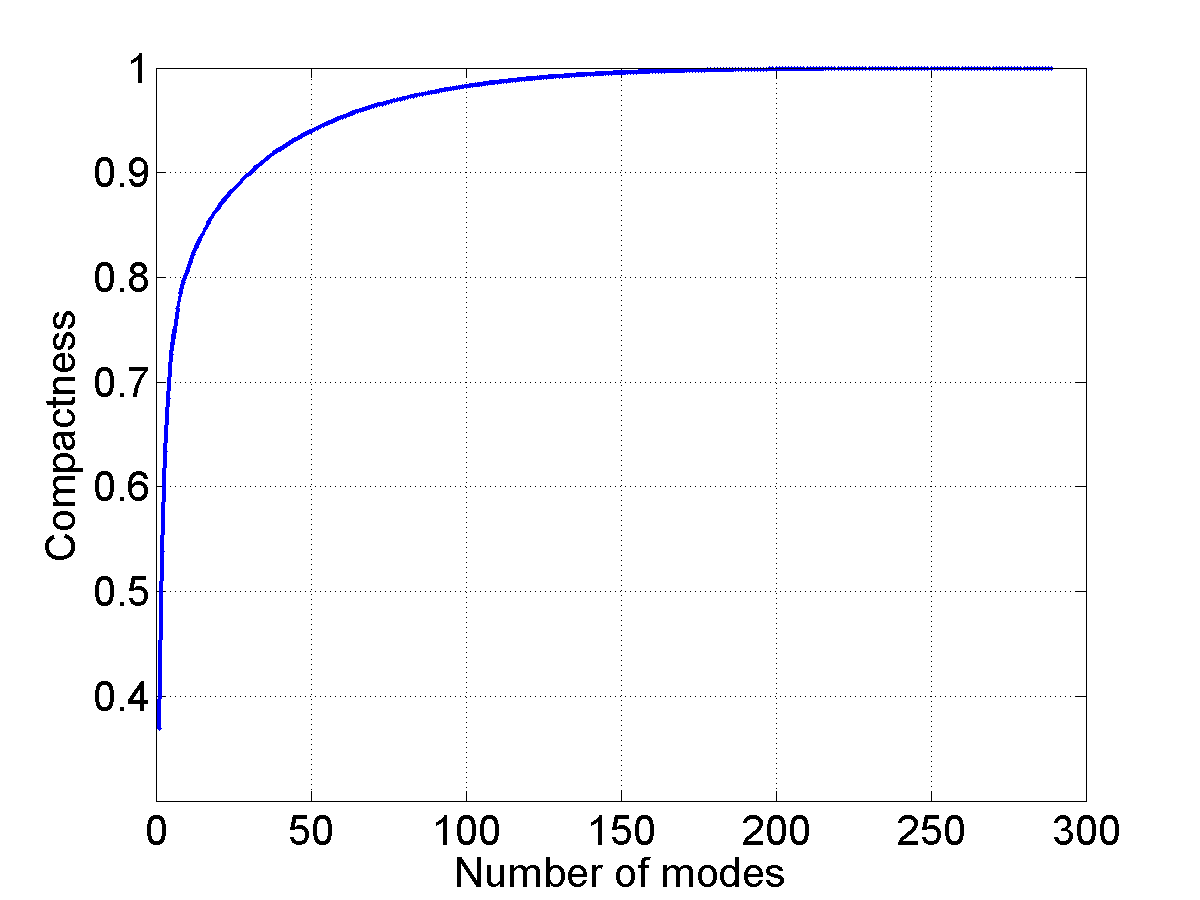
\includegraphics[width=\columnwidth]{images/compactness}
% \caption{Compactness of the constructed SSM given the first $L$ principal modes of variation.}\label{fig:SSM_compactness}
%\end{figure}
%%%%%%%%%%%%%%%%%%%%%%%%%%%%%%%%%